\documentclass[12pt,oneside]{report}

\usepackage[spanish,es-tabla]{babel}
\usepackage[utf8]{inputenc}
\usepackage[T1]{fontenc}
\usepackage[a4paper,top=3cm,bottom=3cm,left=3.5cm,right=2.5cm]{geometry}
\usepackage{setspace}
\usepackage{graphicx}
\usepackage{amsmath,amssymb}
\usepackage{booktabs}
\usepackage{array}
\usepackage{longtable}
\usepackage{pdflscape}
\usepackage{csquotes}
\usepackage[authoryear,round]{natbib}
\usepackage{hyperref}
\usepackage{tocbibind}

\hypersetup{
  colorlinks=true,
  linkcolor=black,
  citecolor=black,
  urlcolor=black,
  pdftitle={Título de la tesis},
  pdfauthor={Nombre del autor}
}

\onehalfspacing
\setlength{\parindent}{1.25cm}
\setlength{\parskip}{0.5\baselineskip}

\begin{document}

\pagenumbering{gobble}
\begin{titlepage}
  \centering
  {\Large \textbf{Universidad Nacional Mayor de San Marcos}}\\[0.4cm]
  {\large Universidad del Perú, Decana de América}\\[0.4cm]
  {\large Facultad de \textit{Nombre de la facultad}}\\[0.2cm]
  {\large Escuela Profesional de \textit{Nombre de la escuela}}\\[1.8cm]

  % Si tienes el escudo de la universidad, guárdalo en el proyecto y reemplaza la línea siguiente.
  % \includegraphics[width=0.25\textwidth]{escudo-unmsm.png}\\[1.5cm]

  {\Large \textbf{Título de la tesis}}\\[1.5cm]

  {\large Tesis para optar el título profesional de \textit{Nombre del título profesional}}\\[1.2cm]

  {\large \textbf{Autor}}\\[0.2cm]
  {\large Tomasto Solis, Victor Eduardo}\\[0.8cm]

  {\large \textbf{Asesor}}\\[0.2cm]
  {\large Canepa Perez, Carlos Alberto}\\[1.5cm]

  {\large Lima, Perú}\\[0.2cm]
  {\large 2026}
\end{titlepage}

\clearpage
\pagenumbering{roman}

\chapter*{Dedicatoria}
\addcontentsline{toc}{chapter}{Dedicatoria}
Escribe aquí una dedicatoria breve y personal.

\chapter*{Agradecimientos}
\addcontentsline{toc}{chapter}{Agradecimientos}
Escribe aquí los agradecimientos a personas, instituciones, laboratorios, proyectos o fuentes de financiamiento que apoyaron el desarrollo de la investigación.

\chapter*{Resumen}
\addcontentsline{toc}{chapter}{Resumen}
El resumen debe presentar de forma concisa el problema de investigación, el objetivo general, la metodología, los principales resultados y las conclusiones. Se recomienda redactarlo en un solo bloque, con lenguaje claro y académico.

\textbf{Palabras clave:} 3D Gaussian Splatting; reconstrucción tridimensional; autoconstrucción; evaluación estructural; inspección digital.

\chapter*{Abstract}
\addcontentsline{toc}{chapter}{Abstract}
The abstract should briefly state the research problem, general objective, methodology, main findings, and conclusions.

\textbf{Keywords:} 3D Gaussian Splatting; three-dimensional reconstruction; self-built housing; structural assessment; digital inspection.

\tableofcontents
\listoffigures
\listoftables

\clearpage
\pagenumbering{arabic}

\chapter{Introducción}

\section{Antecedentes}
El acceso a una vivienda segura y adecuada continúa siendo uno de los principales desafíos urbanos en América Latina, particularmente en países como el Perú, donde el crecimiento acelerado de las ciudades ha superado la capacidad del Estado y del mercado formal para atender la demanda habitacional. Ante esta limitación estructural, millones de familias recurren a soluciones por cuenta propia para edificar sus viviendas, levantando estructuras de manera progresiva y muchas veces sin asistencia técnica especializada. Este fenómeno, extendido en las periferias urbanas desde hace varias décadas, ha configurado gran parte del tejido urbano actual y constituye tanto una estrategia de supervivencia como una fuente significativa de riesgos estructurales y de habitabilidad. Es en este contexto donde cobra relevancia la comprensión del proceso de autoconstrucción y sus implicancias para la seguridad y resiliencia de las viviendas en el país.\par

La autoconstrucción se define como la autogestión del hábitat de manera informal; es un concepto asociado a la forma de edificar en zonas periurbanas que comprende procesos como el diseño, la autogestión de materiales y recursos, la utilización de métodos de autoayuda y la construcción progresiva ajustada a la capacidad económica del hogar (Castro \& Perdomo, 2024). Esta forma de edificación supone un riesgo tanto para quienes la practican como para su entorno, pues al prescindir de la asesoría profesional y de la supervisión técnica adecuada, las construcciones suelen presentar deficiencias estructurales que incrementan su vulnerabilidad frente a eventos naturales. El Perú, por su condición geográfica y su ubicación en el Cinturón de Fuego del Pacífico, está expuesto a una alta sismicidad y a fenómenos climatológicos como inundaciones y huaycos, entre otros; estas condiciones agravan aún más los riesgos de colapso de edificaciones autoconstruidas y evidencian la necesidad de promover viviendas seguras y técnicamente planificadas. \par

En países del Sur Global, como los ubicados en Latinoamérica, África y Asia, la autoconstrucción informal surge como respuesta al déficit habitacional, la pobreza urbana y la burocracia estatal. En contraste, en el Norte Global la autoconstrucción puede desarrollarse de manera planificada, con apoyo de cooperativas, marcos regulatorios o programas específicos, como ocurre con experiencias de \textit{self-build housing} en países como Reino Unido o Alemania (Murillo, 2012). En ese sentido, la construcción surge como una solución al hábitat y presenta variaciones incluso dentro de un mismo país o comunidad, como se muestra en la Figura~\ref{fig:factores-autoconstruccion}.

\begin{figure}[htbp]
  \centering
  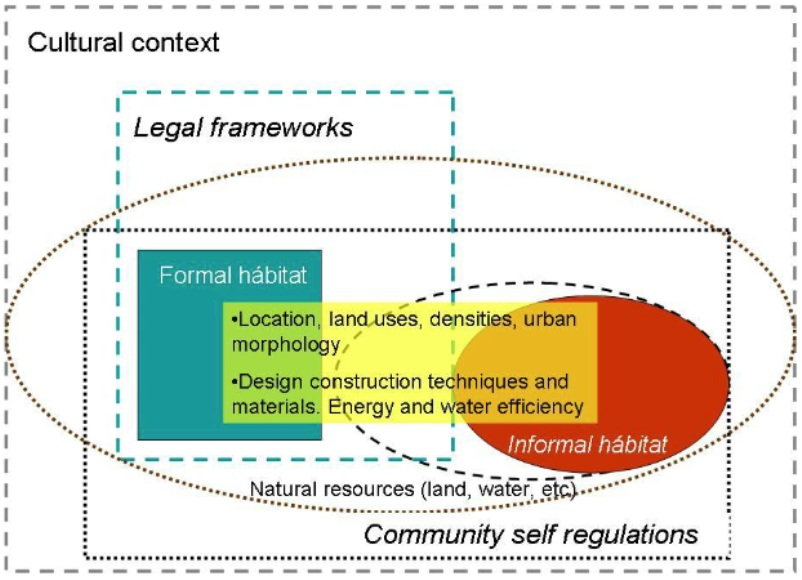
\includegraphics[width=0.8\textwidth]{figuras/figura1.1.jpg}
  \caption{Combinación de factores sobre la autoconstrucción.}
  \label{fig:factores-autoconstruccion}
  \vspace{0.2cm}

  \small \textit{Fuente:} Extraído de Murillo (2012).
\end{figure} 

En América Latina y el Caribe, según el Reporte de Economía y Desarrollo 2017 de CAF (RED 2017), si los hogares latinoamericanos destinaran el 30\% de sus ingresos al consumo de servicios habitacionales, necesitarían más de 30 años de ahorro para adquirir una vivienda de 60~m$^2$ de precio mediano. En ese contexto, la proliferación de asentamientos precarios en la región constituye una expresión extrema de las limitaciones del mercado de vivienda para responder a este déficit. \par

En Chile, Malatesta (2007) propuso un modelo de comunicación informático aplicado a la producción social del hábitat, con el fin de fortalecer los procesos de autoconstrucción mediante la teleformación de los usuarios. La propuesta se basó en un sistema de ayuda informatizada orientado a transmitir conocimientos técnicos de manera asincrónica a los autoconstructores, validado mediante la usabilidad y pertinencia temática del portal desarrollado. Esta investigación demostró la persistencia de la autoconstrucción en sectores populares y la necesidad de incorporar herramientas tecnológicas que respeten las dinámicas sociales del hábitat popular. Sin embargo, su enfoque se centró principalmente en la educación y capacitación, dejando abierta la posibilidad de explorar soluciones basadas en diagnóstico automatizado y modelado digital, como las que propone la presente investigación. \par

En Brasil, la autoconstrucción constituye una práctica extendida entre los sectores de bajos ingresos, vinculada a la falta de acceso a servicios técnicos especializados. Según Luz da Conceição (2023), la ausencia de asistencia técnica en este tipo de edificaciones ha favorecido la proliferación de asentamientos precarios sin condiciones adecuadas de habitabilidad. En respuesta a esta problemática, se han impulsado iniciativas estatales orientadas a reducir la distancia entre el conocimiento técnico y las prácticas empíricas de construcción, como la Asistencia Técnica para la Vivienda de Interés Social (ATHIS). Sin embargo, pese a los avances obtenidos, los resultados muestran que la cobertura sigue siendo limitada frente a la magnitud del déficit habitacional y la informalidad constructiva existente.\par

En Colombia, se han implementado esfuerzos orientados a mejorar la gestión técnica y administrativa en los procesos de acceso a vivienda formal. Ardila Itriago (2018) documenta una experiencia desarrollada en la Caja de Compensación CAJASAN, donde la asistencia técnica y administrativa en visitas de vivienda nueva, usada o en mejoramiento permitió incrementar la cantidad de subsidios aprobados. Este resultado se logró mediante una comunicación más eficiente y una entrega detallada de información a los solicitantes, lo que evidencia la relevancia de los mecanismos de acompañamiento técnico en la reducción de errores y la formalización del proceso constructivo.\par

En el Perú, la autoconstrucción representa una modalidad preponderante de acceso a la vivienda. De acuerdo con un estudio realizado por GRADE para ADI Perú, aproximadamente el 71\% de las viviendas ubicadas en zonas urbanas del país han sido levantadas bajo esquemas de autoconstrucción o edificación progresiva (GRADE, 2023). Esto se manifiesta con mayor intensidad en ciudades intermedias y periferias de Lima Metropolitana, donde las oportunidades de vivienda formal son limitadas. Esta elevada incidencia indica claramente que la autoconstrucción no solo es una alternativa habitacional, sino también un fenómeno estructural del mercado de vivienda peruano, con implicancias directas en la seguridad, la planificación urbana y la gestión de riesgos estructurales, como se muestra en la Figura~\ref{fig:viviendas-autoconstruidas}.

\begin{figure}[htbp]
  \centering
  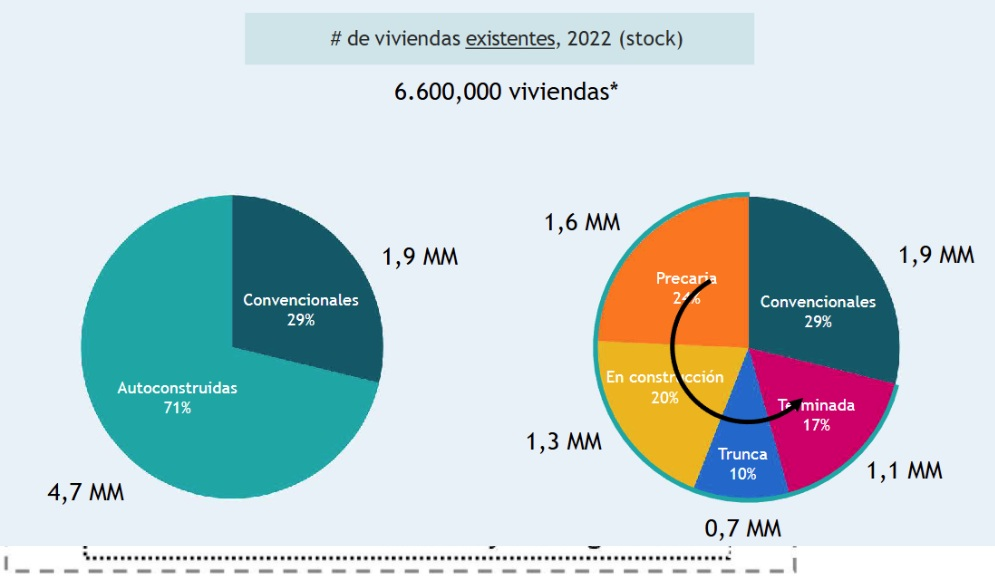
\includegraphics[width=0.8\textwidth]{figuras/figura1.2.jpg}
  \caption{Número de viviendas autoconstruidas.}
  \label{fig:viviendas-autoconstruidas}
  \vspace{0.2cm}

  \small \textit{Fuente:} GRADE (2023).
\end{figure}

En el Perú, el Ministerio de Vivienda, Construcción y Saneamiento advierte sobre la gravedad del proceso informal mediante el cual se han construido numerosas viviendas en nuevos distritos y asentamientos humanos. Estas edificaciones suelen levantarse sin conocimientos técnicos suficientes y con materiales inapropiados para el tipo de vivienda, lo que incrementa su vulnerabilidad frente a desastres naturales. Según datos del INEI, solo el 16\% de las viviendas informales contó con licencia de construcción y apenas el 14\% fue construida con asistencia de un ingeniero civil o arquitecto. En su defecto, la mayoría de estas viviendas recurre a maestros de obra, quienes representan una alternativa menos costosa, pero no siempre cuentan con los conocimientos técnicos necesarios para garantizar estructuras seguras y resistentes, como se muestra en la Figura~\ref{fig:calidad-estructural-viviendas-informales}.

\begin{figure}[htbp]
  \centering
  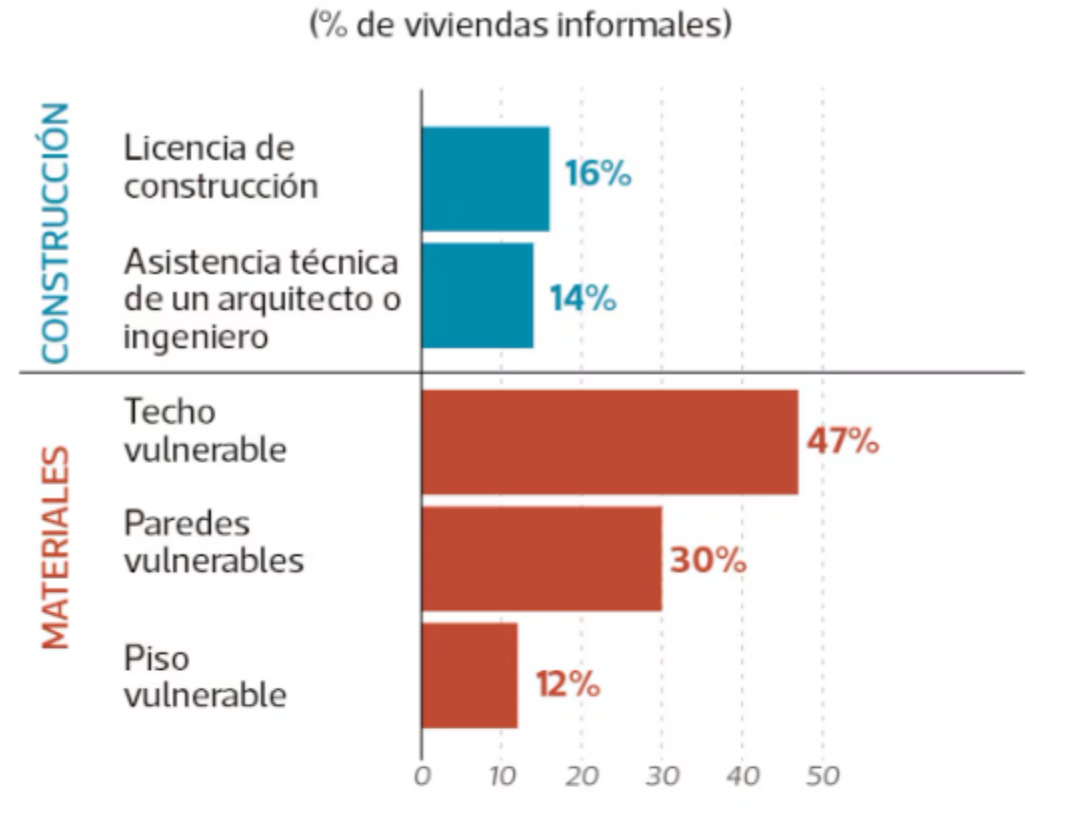
\includegraphics[width=0.8\textwidth]{figuras/figura1.3.jpg}
  \caption{Indicadores de calidad estructural de las viviendas informales en Lima.}
  \label{fig:calidad-estructural-viviendas-informales}
  \vspace{0.2cm}

  \small \textit{Nota:} Se consideran vulnerables las viviendas con pisos de materiales distintos al cemento, madera, losetas, terrazos o láminas; paredes de materiales distintos al ladrillo o piedra unida con cal o cemento; y techos de materiales no adecuados para la seguridad estructural.

  \small \textit{Fuente:} INEI (2024), Indicadores de calidad estructural de las viviendas informales en Lima.
\end{figure}

Chumpitaz Martínez (2023) propone un programa municipal de asistencia técnica orientado a la construcción progresiva de viviendas autoconstruidas en Lima Metropolitana. La investigación combina un enfoque documental y de campo para caracterizar las tipologías de vivienda autoconstruida y definir modalidades de asistencia técnica adecuadas a cada contexto. El estudio plantea la creación del Programa Municipal para la Construcción Asistida de Viviendas Progresivas y Autoconstruidas (PCA) y desarrolla un proyecto piloto en el sector La Flor, Carabayllo, que busca articular el trabajo entre el gobierno local y la ciudadanía mediante un modelo de cogobernanza habitacional. Entre sus conclusiones, el autor destaca la necesidad de complementar la focalización poblacional con la focalización territorial, integrando criterios de habitabilidad, entorno urbano y organización social, como base para políticas sostenibles de vivienda social asistida.\par

Flores Laurente y Urure Rojas (2024) desarrollaron un plan de asistencia técnica para reducir la vulnerabilidad estructural en viviendas autoconstruidas de dos pisos en el distrito de Ciudad Nueva, Tacna. La investigación se basó en observación directa, encuestas y análisis documental, aplicadas a 28 pobladores y 5 viviendas autoconstruidas, lo que permitió identificar las principales deficiencias en diseño y construcción. Los resultados evidenciaron que el 39,2\% de los encuestados no contó con asesoría profesional durante las etapas de diseño arquitectónico, estructural, sanitario o eléctrico, y un porcentaje similar tampoco recibió orientación técnica durante la ejecución de la obra. Asimismo, se reportó que más del 78\% de las viviendas presentaban deterioro en columnas y cerca del 21\% en vigas y muros. Estas deficiencias estructurales aumentan el riesgo de colapso ante un evento sísmico, destacando la necesidad de implementar estrategias de acompañamiento técnico y programas de asistencia preventiva que garanticen la seguridad de las familias y la sostenibilidad de las edificaciones autoconstruidas en el país.\par

En el contexto de la informalidad constructiva, la verificación estructural de viviendas autoconstruidas en el Perú depende casi exclusivamente de inspecciones presenciales realizadas por ingenieros municipales o consultores privados. Este proceso, además de ser costoso y poco accesible para familias de bajos recursos, presenta limitaciones operativas importantes: la cobertura técnica es reducida y la mayoría de distritos no cuenta con personal especializado o herramientas digitales que permitan evaluar de forma rápida la seguridad estructural de una vivienda existente. Según SENCICO (2023), más del 60\% de las viviendas autoconstruidas del país no han pasado por una revisión técnica formal, lo que incrementa su vulnerabilidad frente a sismos o fallas de cimentación.\par

Frente a ello, en los últimos años se ha extendido el uso de técnicas de análisis no destructivo (NDT, por sus siglas en inglés) que permiten estimar la calidad y estabilidad de las edificaciones sin necesidad de intervenir físicamente en la estructura. Entre las más comunes se encuentran la termografía infrarroja, el escaneo láser 3D, el ultrasonido de concreto y la fotogrametría digital (Gao et al., 2023). Estas herramientas ofrecen ventajas al proporcionar modelos tridimensionales del inmueble y detectar deformaciones o irregularidades geométricas. Sin embargo, su aplicación en el contexto peruano sigue siendo limitada por el alto costo del equipamiento, la complejidad del procesamiento de datos y la falta de personal técnico capacitado para interpretar los resultados (Flores \& Urure, 2024).\par

En este escenario emerge el potencial de 3D Gaussian Splatting (3DGS) para representar escenas capturadas mediante imágenes y visualizar nuevas vistas con alta calidad y renderizado en tiempo real \citep{kerbl2023}. Esta propiedad del renderizado no implica que la reconstrucción ni la preparación de los datos se ejecuten en tiempo real. El procedimiento considera la estimación de parámetros de cámara y una representación inicial de la escena. Para las capturas previstas con dron e iPhone se documentarán por separado los dispositivos, las lentes, la resolución y los parámetros disponibles; el procesamiento deberá considerar las características de cada cámara \citep{colmaptutorial}.\par

En la solución propuesta, el análisis mediante inteligencia artificial se aplicará a fotografías y fotogramas para identificar las categorías de deficiencias observables seleccionadas. Las detecciones se asociarán posteriormente con la representación tridimensional mediante un procedimiento de correspondencia espacial cuya exactitud deberá evaluarse. Esta secuencia distingue la identificación en imágenes de la localización de hallazgos en 3D y permite conservar la evidencia visual que sustenta cada resultado.\par

La investigación propone un prototipo que utilice capturas exteriores mediante dron e interiores mediante iPhone para construir representaciones tridimensionales y localizar deficiencias observables identificadas mediante inteligencia artificial. El sistema buscará apoyar la revisión preliminar de las viviendas mediante evidencias trazables, visualización y reportes. Su evaluación se centrará en el desempeño de la reconstrucción, la identificación y la localización de hallazgos, sin atribuir a las imágenes por sí solas la capacidad de determinar la distribución de cargas o la seguridad estructural integral de una vivienda.\par


\section{Definición del problema}
La investigación aborda la integración de datos visuales obtenidos en viviendas autoconstruidas, reconstrucción tridimensional e inteligencia artificial en un flujo de apoyo a la identificación de deficiencias constructivas observables. El problema se delimita a la obtención y preparación de datos, la representación tridimensional de los elementos de interés, la identificación y localización de hallazgos y la evaluación del desempeño del prototipo. A partir de esta delimitación se formulan las siguientes preguntas de investigación.

\subsection{Problema general}
¿Cómo desarrollar y evaluar un prototipo tecnológico que integre reconstrucción tridimensional mediante 3D Gaussian Splatting e inteligencia artificial para apoyar la identificación de deficiencias constructivas observables en viviendas autoconstruidas, a partir de datos visuales capturados en condiciones reales?

\subsection{Problemas específicos}
\begin{enumerate}
  \item ¿Qué deficiencias constructivas observables, requisitos de información y criterios de evaluación deben considerarse para orientar el desarrollo del prototipo?
  \item ¿Cómo obtener y preparar un conjunto de datos visuales mediante captura exterior con dron e interior con iPhone en viviendas autoconstruidas reales, para desarrollar y evaluar la reconstrucción tridimensional y la identificación de deficiencias constructivas?
  \item ¿Cómo reconstruir tridimensionalmente las viviendas mediante 3D Gaussian Splatting, a partir de los datos visuales preparados, para visualizar y localizar los elementos de interés?
  \item ¿Cómo identificar las deficiencias constructivas seleccionadas en fotografías y fotogramas mediante inteligencia artificial y asociar sus detecciones con la representación tridimensional de la vivienda?
  \item ¿Qué desempeño presenta el prototipo en términos de calidad de reconstrucción, detección y localización de deficiencias constructivas y tiempo de procesamiento, respecto de los datos de referencia y criterios de evaluación definidos?
\end{enumerate}

\clearpage
\section{Objetivos}

\subsection{Objetivo general}
Desarrollar y evaluar un prototipo tecnológico que integre reconstrucción tridimensional mediante 3D Gaussian Splatting e inteligencia artificial para apoyar la identificación de deficiencias constructivas observables en viviendas autoconstruidas, a partir de datos visuales capturados en condiciones reales.

\subsection{Objetivos específicos}
\begin{enumerate}
  \item Definir las deficiencias constructivas observables, los requisitos de información y los criterios de evaluación del prototipo, mediante revisión documental y criterios técnicos sustentados.
  \item Construir un conjunto de datos visuales de viviendas autoconstruidas reales mediante captura exterior con dron e interior con iPhone, aplicando protocolos de adquisición, selección, preprocesamiento y anotación de fotografías y fotogramas, para desarrollar y evaluar la reconstrucción tridimensional y la identificación de deficiencias constructivas.
  \item Implementar un procedimiento de reconstrucción tridimensional mediante 3D Gaussian Splatting, a partir de los datos visuales preparados, que permita visualizar y localizar los elementos de interés de las viviendas autoconstruidas.
  \item Integrar un modelo de inteligencia artificial para identificar las deficiencias constructivas seleccionadas en fotografías y fotogramas y asociar sus detecciones con la representación tridimensional de la vivienda dentro del prototipo.
  \item Evaluar el desempeño del prototipo en términos de calidad de reconstrucción, detección y localización de deficiencias constructivas y tiempo de procesamiento, mediante datos de referencia, métricas y criterios de evaluación definidos previamente y un protocolo reproducible.
\end{enumerate}

\section{Justificación}
En el Perú, la autoconstrucción representa una práctica extendida y culturalmente arraigada, especialmente en zonas urbanas y periurbanas donde el acceso a la vivienda formal es limitado. Sin embargo, esta modalidad de edificación suele realizarse sin asesoría técnica profesional, lo que genera viviendas vulnerables ante eventos sísmicos, deslizamientos o lluvias intensas. Según el Ministerio de Vivienda, Construcción y Saneamiento (MVCS 2023), más del 70\% del parque habitacional peruano ha sido construido de manera informal, y cerca del 60\% presenta algún tipo de deficiencia estructural.\par

Frente a esta realidad, el fortalecimiento de los mecanismos de evaluación técnica resulta esencial para reducir la vulnerabilidad estructural de millones de viviendas. No obstante, la supervisión presencial por parte de ingenieros o fiscalizadores resulta limitada debido a la escasez de personal técnico, la dispersión geográfica y los costos asociados. En este contexto, la incorporación de herramientas digitales y modelos de inteligencia artificial se presenta como una alternativa viable y sostenible para apoyar los procesos de inspección y diagnóstico estructural.\par

La combinación de capturas exteriores con dron e interiores con iPhone permitirá reunir evidencias visuales complementarias de las viviendas seleccionadas. Su integración con reconstrucción tridimensional e inteligencia artificial se orientará a identificar y localizar deficiencias observables para apoyar la revisión técnica. La calidad geométrica, el desempeño de detección y los recursos de procesamiento se evaluarán mediante el protocolo experimental, en lugar de asumir su cumplimiento por la elección de la tecnología.\par

Este estudio busca contribuir al desarrollo de un sistema digital que combine reconstrucción 3D y aprendizaje automático para mejorar la gestión técnica de la autoconstrucción, aportando así a la seguridad habitacional y a la reducción del riesgo estructural en el país. Además, constituye una base metodológica para futuras investigaciones en el campo de la ingeniería civil asistida por inteligencia artificial y la modernización de los mecanismos de fiscalización urbana.\par

\section{Importancia}
La autoconstrucción constituye uno de los principales mecanismos de acceso a la vivienda en el Perú, pero también una de las causas más críticas de vulnerabilidad estructural. Según el Ministerio de Vivienda, Construcción y Saneamiento (MVCS, 2023), más del 70\% de las viviendas en el país se levantan sin asistencia técnica profesional, lo que incrementa significativamente el riesgo de colapso durante eventos sísmicos o climáticos.\par

Contar con un sistema digital que organice capturas exteriores e interiores, identifique deficiencias observables en las imágenes y permita consultar su localización en una representación tridimensional aportaría un flujo trazable para la revisión técnica. La contribución de la investigación se evaluará a partir de los resultados del prototipo y de las condiciones de los casos estudiados.\par

La implementación de herramientas de reconstrucción 3D e inteligencia artificial no solo representa un aporte tecnológico al campo de la ingeniería civil, sino que también constituye una estrategia de inclusión social al facilitar el acceso a evaluaciones técnicas precisas, incluso en zonas donde no se dispone de especialistas. En este sentido, la investigación busca contribuir al fortalecimiento de la seguridad habitacional, la sostenibilidad urbana y la modernización de la gestión pública en materia de vivienda.\par

\section{Alcance del prototipo}
El alcance de la presente investigación comprende el desarrollo y la evaluación del prototipo SE-PEAV, desde la captura de datos visuales en viviendas autoconstruidas reales hasta la reconstrucción tridimensional, la identificación de deficiencias constructivas mediante inteligencia artificial y la presentación de hallazgos localizados. La reconstrucción mediante 3D Gaussian Splatting y la integración del modelo de inteligencia artificial constituyen componentes centrales que deberán implementarse y evaluarse. El prototipo apoyará la evaluación preliminar de las deficiencias observables seleccionadas; no sustituirá el juicio profesional de un ingeniero civil ni constituirá un dictamen estructural oficial.\par

La adquisición prevista comprende fotografías y videos del exterior mediante dron y del interior mediante iPhone. Cada sesión se identificará por vivienda, zona, dispositivo y fecha. Se establecerán protocolos diferenciados de recorrido, cobertura, calidad visual y organización de archivos. El alcance considera imágenes RGB; la captura de profundidad o LiDAR no forma parte del procedimiento previsto. El modelo del dron y del iPhone, la aplicación de captura y los parámetros de adquisición se documentarán antes de la recolección, sin fijar una resolución o telemetría que aún no se haya verificado.\par

La preparación incluirá selección de imágenes, extracción de fotogramas cuando corresponda, preprocesamiento, organización de metadatos y anotación de las deficiencias seleccionadas. Las anotaciones deberán contar con criterios documentados y revisión técnica. Las particiones destinadas al entrenamiento o ajuste, la validación y la prueba del modelo de detección se separarán por vivienda, conservando juntos los registros exteriores e interiores de cada inmueble. La evaluación de nuevas vistas de una reconstrucción utilizará imágenes reservadas de esa escena y se distinguirá de la evaluación de la capacidad del detector para generalizar a viviendas no utilizadas en su ajuste. El tamaño y la composición de los conjuntos se documentarán a partir de la captura realizada.\par

Los registros exteriores e interiores se vincularán a una misma vivienda y conservarán la identificación de sus reconstrucciones y sistemas de coordenadas. La decisión de presentar modelos separados o una representación unificada se resolverá mediante pruebas de correspondencia y alineación. La integración geométrica, cuando sea viable, requerirá documentar la transformación entre modelos, la referencia de escala y el error de alineación; no se asumirá una fusión automática por reunir los archivos de ambas capturas.\par

El prototipo integrará servicios de registro y almacenamiento, reconstrucción tridimensional, inferencia mediante inteligencia artificial, asociación de detecciones con la representación tridimensional, visualización y generación de reportes. La selección, adaptación o ajuste del modelo se sustentará en las categorías de deficiencias y los datos disponibles; no se establece como requisito entrenar un modelo desde cero. La evaluación empleará datos de referencia y métricas definidas antes de interpretar los resultados. La captura LiDAR, una aplicación móvil completa y el despliegue en producción quedan fuera del alcance de esta investigación.\par

\section{Limitaciones}

\subsection{Limitación espacial}
El estudio se enfocará en viviendas autoconstruidas de zonas urbanas y periurbanas, priorizando el distrito de Carabayllo, en Lima Metropolitana. La selección de los casos y las condiciones de acceso para la captura se documentarán en el protocolo de recolección de datos.

\subsection{Limitación social}
El prototipo estará orientado principalmente a fiscalizadores municipales, maestros de obra y estudiantes de ingeniería civil, quienes podrán utilizarlo como herramienta de verificación rápida y apoyo en la supervisión de edificaciones.

\subsection{Limitación técnica}
La evaluación se realizará con registros visuales capturados en viviendas reales y datos de referencia documentados. Se distinguirán las condiciones de captura exterior con dron e interior con iPhone, incluyendo visibilidad de los elementos, iluminación, cobertura, oclusiones y calidad de imagen. Se registrarán las zonas no observadas y los hallazgos cuya localización tridimensional no pueda establecerse de manera verificable. Los resultados estarán delimitados por estas condiciones, las categorías anotadas y los recursos de procesamiento disponibles.\par

La evaluación distinguirá la calidad visual de la reconstrucción, su precisión geométrica cuando se disponga de medidas de referencia y el desempeño en detección y localización de las deficiencias seleccionadas. Las métricas de apariencia visual no se utilizarán por sí solas como evidencia de exactitud dimensional. El cumplimiento de los objetivos se sustentará en resultados medidos, sin inferir una reducción del riesgo estructural a escala nacional a partir del funcionamiento del prototipo.\par

\section{Organización de la tesis}
La presente tesis está estructurada en seis capítulos:\par

Capítulo I: Planteamiento metodológico
Describe los antecedentes, formulación del problema, objetivos, justificación, alcance, hipótesis, variables y la organización general del trabajo.\par

Capítulo II: Estado del Arte
Presenta la revisión sistemática de literatura sobre análisis no destructivos en edificaciones, evolución de técnicas de reconstrucción 3D (fotogrametría, NeRF y 3DGS), así como aplicaciones relacionadas en ingeniería civil y arquitectura.\par

Capítulo III: Marco Teórico
Define los conceptos fundamentales asociados al problema (autoconstrucción, predimensionamiento estructural, RNE) y a la solución propuesta (computación gráfica neuronal, 3DGS, métricas de calidad visual y precisión geométrica).\par

Capítulo IV: Metodología de investigación
Detalla el tipo y diseño de la investigación, población y muestra, técnicas de recolección de datos, construcción del dataset, implementación del prototipo, y métodos de validación técnica y subjetiva.\par

Capítulo V: Diseño y desarrollo de la solución
Expone el proceso de construcción del prototipo: herramientas utilizadas, dataset, preprocesamiento, reconstrucción con 3DGS, conversión a malla, sistema de análisis y generación de informes.\par

Capítulo VI: Resultados y análisis
Presenta los resultados obtenidos en las pruebas experimentales: precisión de medidas, rendimiento técnico, percepción de usuarios y comparación con técnicas tradicionales.\par

Capítulo VII: Discusión, conclusiones y recomendaciones
Discute los hallazgos, valida las hipótesis, expone las limitaciones y formula recomendaciones para futuros trabajos.\par

\chapter{Estado del arte}

\section{Metodología de la investigación}
La metodología de este estudio se desarrolló mediante una revisión sistemática de la literatura (RSL) basada en el enfoque propuesto por Kitchenham y Charters (2007), el cual estructura el proceso en tres etapas principales: planificación, desarrollo y resultados.\par

Planificación: En esta etapa se formularon preguntas de investigación orientadas a identificar las técnicas y enfoques más relevantes de reconstrucción tridimensional (3D) aplicadas a la ingeniería civil, arquitectura y análisis estructural. Se buscó determinar los algoritmos, frameworks y modelos de aprendizaje profundo más utilizados, así como los datasets y métricas de evaluación empleados en la literatura reciente. Además, se seleccionaron los repositorios académicos, se definieron las cadenas de búsqueda y se establecieron los criterios de inclusión y exclusión de los artículos analizados.\par

Desarrollo: En esta etapa se ejecutó la búsqueda sistemática en los repositorios seleccionados, aplicando los criterios de elegibilidad definidos. Los artículos fueron revisados y clasificados de acuerdo con su relevancia temática, año de publicación y aporte metodológico. Posteriormente, se organizó la información de manera estructurada para dar respuesta a las preguntas de investigación planteadas.\par

Resultados: Finalmente, se elaboró una síntesis crítica y comparativa de la información recopilada, destacando los principales avances y limitaciones de las técnicas de reconstrucción 3D, con especial atención a la evolución desde la fotogrametría tradicional y NeRF hasta la implementación de 3D Gaussian Splatting (3DGS) y su potencial aplicación en la fiscalización técnica de edificaciones y análisis no destructivo.\par


\section{Planificación de la revisión}

\subsection{Preguntas de investigación}
Se llevó a cabo una revisión bibliográfica exhaustiva con el objetivo de recopilar información actualizada sobre las técnicas y métodos empleados en la reconstrucción tridimensional de escenas y edificaciones mediante inteligencia artificial y renderizado neuronal.\par

En primer lugar, se formularon preguntas específicas destinadas a comprender el estado actual de las tecnologías aplicadas a la reconstrucción 3D, su evolución hacia modelos basados en 3D Gaussian Splatting (3DGS) y su potencial aplicación en el análisis no destructivo de estructuras civiles.\par

Cada pregunta se centra en un aspecto técnico o metodológico clave de las soluciones basadas en IA y visión por computadora, y sus respuestas son fundamentales para definir el alcance de la presente investigación.\par

Se plantearon las siguientes preguntas de investigación:\par

Q1: ¿Cuáles son las técnicas o métodos actuales de reconstrucción 3D empleados en ingeniería civil y arquitectura?\par

Q2: ¿Qué ventajas y limitaciones presenta 3D Gaussian Splatting frente a otros enfoques como Neural Radiance Fields (NeRF) y la fotogrametría tradicional?\par

Q3: ¿Qué datasets o fuentes de datos se utilizan comúnmente para el entrenamiento y validación de modelos de reconstrucción tridimensional?\par

Q4: ¿Cuáles son las métricas más relevantes para evaluar la calidad visual y geométrica de las reconstrucciones tridimensionales?\par

Q5: ¿Qué aplicaciones concretas del 3DGS existen en el ámbito de la ingeniería civil, arquitectura o fiscalización técnica de edificaciones?\par

\subsection{Repositorio y proceso de búsqueda}
Para seleccionar los repositorios académicos, se consideraron aspectos como la cobertura temática y la especialización en áreas de ingeniería civil, visión por computadora y computación gráfica, así como la calidad y accesibilidad de las publicaciones indexadas.\par

Los repositorios elegidos fueron Scopus, IEEE Xplore, ScienceDirect, SpringerLink y ACM Digital Library, por su relevancia en la difusión de investigaciones relacionadas con la reconstrucción tridimensional, el renderizado neuronal y la aplicación de inteligencia artificial en ingeniería.\par

Antes de iniciar la búsqueda, se diseñaron cadenas de consulta específicas para cada repositorio, utilizando combinaciones de palabras clave tales como “3D Gaussian Splatting”, “Neural Radiance Fields”, “3D reconstruction”, “photogrammetry”, “non-destructive evaluation”, “structural inspection”, “LiDAR”, “civil engineering” y “architecture”.\par

\subsection{Criterios de elegibilidad}
Se priorizaron artículos publicados en los últimos cinco años (2020–2025) con el propósito de identificar los avances más recientes en técnicas de reconstrucción tridimensional (3D) y renderizado neuronal aplicadas a la ingeniería civil, arquitectura y análisis estructural.\par

Los criterios definidos permitieron asegurar la relevancia técnica y científica de los trabajos seleccionados, garantizando que los estudios analizados contribuyan de manera significativa al entendimiento y evolución de métodos como 3D Gaussian Splatting (3DGS), Neural Radiance Fields (NeRF) y la fotogrametría avanzada en contextos reales de inspección estructural.\par


\begin{table}[htbp]
  \centering
  \caption{Criterios de inclusión y exclusión de estudios}
  \label{tab:criterios-inclusion-exclusion}
  \small
  \begin{tabular}{p{0.45\textwidth} p{0.45\textwidth}}
    \toprule
    \textbf{Criterios de inclusión} & \textbf{Criterios de exclusión} \\
    \midrule
    \begin{itemize}
      \setlength\itemsep{0.2em}
      \item Artículos publicados entre 2020 y 2025.
      \item Estudios orientados a la reconstrucción tridimensional o al análisis visual de estructuras o escenas reales.
      \item Trabajos que describen o implementan técnicas basadas en aprendizaje profundo, visión por computadora o renderizado neuronal, como NeRF, 3DGS u otros enfoques relacionados.
      \item Investigaciones que responden a una o más de las preguntas de investigación planteadas.
      \item Estudios que incluyen métricas objetivas de rendimiento o calidad visual, tales como PSNR, SSIM, LPIPS, FPS u otras métricas comparables.
    \end{itemize}
    &
    \begin{itemize}
      \setlength\itemsep{0.2em}
      \item Documentos que sean libros, tesis o reportes sin revisión por pares.
      \item Publicaciones cuyo idioma no sea inglés o español.
      \item Revisiones teóricas sin experimentación o validación práctica.
      \item Trabajos enfocados exclusivamente en el ámbito del entretenimiento o videojuegos.
      \item Estudios que no disponen de acceso al texto completo.
    \end{itemize} \\
    \bottomrule
  \end{tabular}
\end{table}

\section{Desarrollo de la revisión}
Una vez seleccionados los repositorios académicos (Scopus, IEEE Xplore, ScienceDirect y ACM Digital Library), se emplearon las palabras clave y cadenas de búsqueda previamente definidas, tales como “3D Gaussian Splatting”, “Neural Radiance Fields”, “3D reconstruction”, “photogrammetry”, “structural analysis”, “civil engineering” y “architectural heritage”.\par

Esta búsqueda inicial dio como resultado 432 artículos potencialmente elegibles. Luego se procedió a aplicar los criterios de exclusión, reduciendo el conjunto a 158 artículos. Posteriormente, se analizaron los resúmenes, conclusiones y secciones experimentales, aplicando los criterios de inclusión definidos en la Tabla 2.2, lo que permitió seleccionar 82 artículos con contenido relevante.\par

Finalmente, tras una revisión completa de los documentos restantes, se identificaron 40 artículos científicos directamente relacionados con los objetivos de esta investigación, los cuales abordan técnicas de reconstrucción 3D, renderizado neuronal y su aplicación en contextos de ingeniería civil y arquitectura.\par

\section{Resultado de la búsqueda}

\begin{landscape}
\scriptsize
\setlength{\tabcolsep}{3pt}
\renewcommand{\arraystretch}{1.15}
\begin{longtable}{>{\raggedright\arraybackslash}p{0.03\linewidth} >{\raggedright\arraybackslash}p{0.27\linewidth} >{\centering\arraybackslash}p{0.05\linewidth} >{\raggedright\arraybackslash}p{0.08\linewidth} >{\raggedright\arraybackslash}p{0.14\linewidth} >{\raggedright\arraybackslash}p{0.15\linewidth} >{\raggedright\arraybackslash}p{0.13\linewidth}}
\caption{Artículos seleccionados para la revisión sistemática}\label{tab:articulos-seleccionados}\\
\toprule
\textbf{N} & \textbf{Título del paper} & \textbf{Año} & \textbf{Fuente} & \textbf{Área de aplicación} & \textbf{Técnica usada} & \textbf{Métricas reportadas} \\
\midrule
\endfirsthead
\caption[]{Artículos seleccionados para la revisión sistemática (continuación)}\\
\toprule
\textbf{N} & \textbf{Título del paper} & \textbf{Año} & \textbf{Fuente} & \textbf{Área de aplicación} & \textbf{Técnica usada} & \textbf{Métricas reportadas} \\
\midrule
\endhead
\midrule
\multicolumn{7}{r}{\small Continúa en la siguiente página}\\
\endfoot
\bottomrule
\endlastfoot
    1 & LiDAR-3DGS: LiDAR reinforcement for multimodal initialization of 3D Gaussian Splats & 2024 & ScienceDirect & Topografía, GIS & 3DGS + LiDAR & SSIM/PSNR, tiempo \\
    2 & Integrating 3DGS novel view synthesis and CFD for modeling bionic robotic fish from multi view imagery & 2024 & ScienceDirect & Robótica, simulación de fluidos & 3DGS + CFD & Error relativo \\
    3 & High-fidelity 3D reconstruction of peach orchards using a 3DGS-Ag model & 2023 & ScienceDirect & Agricultura de precisión & 3DGS & SSIM, reconstrucción \\
    4 & Biomass phenotyping of oilseed rape through UAV multi-view oblique imaging with 3DGS and SAM model & 2024 & ScienceDirect & Agricultura (fenotipado) & 3DGS + UAV & Volumen, error geométrico \\
    5 & A 3DGS and LLM-based physical-to-virtual approach for human-robot interactive manufacturing & 2024 & ScienceDirect & Industria 4.0 & 3DGS + LLM & FPS, precisión \\
    6 & From comparison to integration: A workflow evaluation of 3D Gaussian splatting and LiDAR point cloud for modern architectural heritage & 2023 & ScienceDirect & Arquitectura, patrimonio & 3DGS + LiDAR & Comparación tiempo/calidad \\
    7 & 3DGStrands: Personalized 3D Gaussian splatting for realistic hair representation and animation & 2024 & ScienceDirect & Animación, videojuegos & 3DGS & SSIM, FPS \\
    8 & EGU-GS: Efficient Gaussian utilization for real-time 3D Gaussian splatting & 2024 & ScienceDirect & Computación gráfica (optimización) & 3DGS optimizado & FPS, memoria \\
    9 & Highly stretchable and conductive 3D graphene skeleton/polyacrylamide/LiCl nanocomposite hydrogels for high-performance electromagnetic interference shielding & 2023 & ScienceDirect & Materiales & 3D graphene skeleton & N/A \\
    10 & SHREC GS-3DORC: Towards the advancements of 3D Gaussian Splatting object part retrieval & 2023 & ScienceDirect & Visión por computadora (dataset retrieval) & 3DGS & Accuracy retrieval \\
    11 & Regularized three-dimensional Gaussians for large-scale building reconstruction with spatial prior & 2024 & ScienceDirect & Arquitectura / civil & 3DGS & Error geométrico, SSIM \\
    12 & A review of recent advances in 3D Gaussian Splatting for optimization and reconstruction & 2024 & ScienceDirect & Revisión general & 3DGS & FPS \\
    13 & Cotton3DGaussians: Multiview 3D Gaussian Splatting for boll mapping and plant architecture analysis & 2023 & ScienceDirect & Agricultura & 3DGS & Volumen, error \\
    14 & FastTalker: Real-time audio-driven talking face generation with 3D Gaussian & 2024 & ScienceDirect & IA / animación & 3DGS & FPS, calidad visual \\
    15 & FeatureGS: Eigenvalue-feature optimization in 3D Gaussian Splatting for geometrically accurate and artifact-reduced reconstruction & 2024 & ScienceDirect & Computación gráfica & 3DGS & Error geométrico, SSIM \\
    16 & Novel UAV-based 3D reconstruction using dense LiDAR point cloud and imagery: A geometry-aware 3D gaussian splatting approach & 2024 & ScienceDirect & Ingeniería civil, topografía & 3DGS + LiDAR & Error relativo, SSIM \\
    17 & P3DFusion: A cross-scene and high-fidelity 3D plant reconstruction framework empowered by vision foundation models and 3D Gaussian splatting & 2024 & ScienceDirect & Agricultura & 3DGS + foundation models & SSIM, PSNR \\
    18 & LFGS: A lightweight framework for efficient 3D Gaussian Splatting with minimal memory footprint & 2024 & ScienceDirect & Computación gráfica & 3DGS & FPS, memoria \\
    19 & PcdGS: A point cloud densification method for Gaussian Splatting & 2024 & ScienceDirect & Visión 3D & 3DGS & Densidad, error geométrico \\
    20 & A Neural Rendering system for fashion design process & 2024 & ScienceDirect & Moda / diseño & 3DGS & Calidad visual \\
    21 & USGS: Enhancing sparse view synthesis with unseen viewpoint regularization in 3D Gaussian splatting & 2024 & ScienceDirect & Computación gráfica & 3DGS & SSIM, LPIPS \\
    22 & ESA-GS: Elongation splitting and assimilation in Gaussian splatting for accurate surface reconstruction & 2025 & ScienceDirect & Computación gráfica / superficies & 3DGS con elongation splitting & SSIM, error geométrico \\
    23 & SREGS: Sparse-view Gaussian radiance fields with geometric regularization and region exploration & 2025 & ScienceDirect & Reconstrucción con pocas vistas & 3DGS con regularización geométrica & PSNR, SSIM \\
    24 & High-fidelity 3D Gaussian inpainting: Preserving multi-view consistency and photorealistic details & 2025 & ScienceDirect & Reconstrucción + completado de huecos & 3DGS + inpainting multi-view & SSIM, LPIPS \\
    25 & SuraGS: Toward efficient few-shot novel view synthesis via surface-aware Gaussian splatting & 2025 & ScienceDirect & Reconstrucción eficiente & 3DGS + awareness de superficie & SSIM, FPS \\
    26 & UV Gaussians: Joint learning of mesh deformation and Gaussian textures for human avatar modeling & 2025 & ScienceDirect & Animación / modelado humano & 3DGS + malla UV & Calidad de texturas, FPS \\
    27 & DualPhys-GS: Dual physically-guided 3D Gaussian splatting for underwater scene reconstruction & 2025 & ScienceDirect & Medio acuático / visión submarina & 3DGS + guías físicas & SSIM, error de reconstrucción \\
    28 & StruGS: Structurally consistent 3D Gaussian Splatting with targeted optimization strategies & 2025 & ScienceDirect & Ingeniería / arquitectura & 3DGS + optimización estructural & Error geométrico, PSNR \\
    29 & IPENS: Interactive Unsupervised Framework for Rapid Plant Phenotyping Extraction via NeRF-SAM2 Fusion & 2025 & ScienceDirect & Agricultura, plantas & NeRF + SAM2 + visión & Accuracy fenotípica \\
    30 & Multi-view optimization and refinement for high-fidelity 4D Gaussian splatting & 2025 & ScienceDirect & Escenas dinámicas (tiempo) & 4DGS & SSIM, temporal coherence \\
    31 & 4DStyleGaussian: Generalizable 4D Style Transfer with Gaussian Splatting & 2025 & ScienceDirect & Arte / estilo visual & 4DGS + style transfer & Calidad subjetiva \\
    32 & Simulated Skewed Gaussian Splatting: A New Approach to Geometric Primitives & 2025 & Scopus & Visualización 3D, reconstrucción & 3D Gaussian Splatting & Calidad visual, error geométrico \\
    33 & PFGS: Pose-Fused 3D Gaussian Splatting for Complete Multi-Pose Object Reconstruction & 2025 & Scopus & Reconstrucción 3D, visión por computadora & 3D Gaussian Splatting + multi-pose fusion & Fidelidad de reconstrucción, cobertura de pose \\
    34 & SG-Splatting: Accelerating 3D Gaussian Splatting with Spherical Gaussians & 2025 & Scopus & Visualización 3D, renderizado en tiempo real & 3D Gaussian Splatting + Spherical Gaussians & Tiempo de render, calidad visual \\
    35 & 3D Gaussian Splatting: Techniques and Applications in Architecture & 2025 & Scopus & Arquitectura, diseño visual & 3D Gaussian Splatting & Detalle visual, eficiencia \\
    36 & Practical application of Gaussian Splatting with new geometric primitives for modeling constructions & 2025 & Scopus & Ingeniería estructural, reconstrucción & 3D Gaussian Splatting & Precisión estructural, fidelidad \\
    37 & Evaluation of buildings generated with 3D Gaussian Splatting & 2024 & Scopus & Visualización 3D, modelado & 3D Gaussian Splatting & Calidad visual, comparación temporal \\
    38 & Gaussian Splatting Add-on en Evergine para visualización 3D & 2025 & Scopus & Visualización arquitectónica y productiva & 3D Gaussian Splatting + integración software & Interactividad, detalle visual \\
    39 & 3D Gaussian splatting technologies and extensions: A review & 2025 & ScienceDirect & Visión por computadora, renderizado 3D & 3D Gaussian Splatting y extensiones & Calidad visual, fidelidad, velocidad de render \\
    40 & A novel framework utilizing 3D Gaussian Splatting to reconstruct sparse points from drone images & 2025 & ScienceDirect & Topografía, reconstrucción con drones & 3D Gaussian Splatting + fotogrametría & Precisión geométrica, densidad de puntos \\
\end{longtable}
\normalsize
\end{landscape}

\section{Análisis}

\subsection{Q1: ¿Qué enfoques existen para la reconstrucción tridimensional de escenas y edificaciones?}
\begin{table}[htbp]
  \centering
  \caption{Estudios principales considerados para el análisis comparativo}
  \label{tab:estudios-analisis-comparativo}
  \scriptsize
  \setlength{\tabcolsep}{3pt}
  \renewcommand{\arraystretch}{1.15}
  \begin{tabular}{>{\centering\arraybackslash}p{0.045\textwidth} >{\raggedright\arraybackslash}p{0.32\textwidth} >{\centering\arraybackslash}p{0.06\textwidth} >{\raggedright\arraybackslash}p{0.105\textwidth} >{\raggedright\arraybackslash}p{0.16\textwidth} >{\raggedright\arraybackslash}p{0.145\textwidth}}
    \toprule
    \textbf{N.\textsuperscript{o}} & \textbf{Título} & \textbf{Año} & \textbf{Fuente} & \textbf{Técnica} & \textbf{Métricas} \\
    \midrule
    01 & LiDAR-3DGS: LiDAR reinforcement for multimodal initialization of 3D Gaussian Splats & 2024 & Science\-Direct & 3DGS + LiDAR & SSIM/PSNR, tiempo \\
    02 & Biomass phenotyping of oilseed rape through UAV multi-view oblique imaging with 3DGS and SAM model & 2024 & Science\-Direct & 3DGS + UAV & Volumen, error geométrico \\
    03 & FeatureGS: Eigenvalue-feature optimization in 3D Gaussian Splatting for geometrically accurate and artifact-reduced reconstruction & 2024 & Science\-Direct & 3DGS & Error geométrico, SSIM \\
    04 & P3DFusion: A cross-scene and high-fidelity 3D plant reconstruction framework empowered by vision foundation models and 3D Gaussian splatting & 2024 & Science\-Direct & 3DGS + foundation models & SSIM, PSNR \\
    05 & PcdGS: A point cloud densification method for Gaussian Splatting & 2025 & Science\-Direct & Visión 3D & Densidad, error geométrico \\
    06 & UV Gaussians: Joint learning of mesh deformation and Gaussian textures for human avatar modeling & 2025 & Science\-Direct & 3DGS + malla UV & Calidad de texturas, FPS \\
    07 & Practical application of Gaussian Splatting with new geometric primitives for modeling constructions & 2025 & Scopus & 3D Gaussian Splatting & Precisión estructural, fidelidad \\
    08 & 3D Gaussian splatting technologies and extensions: A review & 2025 & Science\-Direct & 3D Gaussian Splatting y extensiones & Calidad visual, fidelidad, velocidad de render \\
    \bottomrule
  \end{tabular}
\end{table}

lorem ipsumlorem ipsumlorem ipsumlorem ipsumlorem ipsumlorem ipsumlorem ipsumlorem ipsumlorem ipsumlorem ipsumlorem ipsumlorem ipsumlorem ipsumlorem ipsumlorem ipsumlorem ipsumlorem ipsumlorem ipsumlorem ipsumlorem ipsumlorem ipsumlorem ipsumlorem ipsumlorem ipsumlorem ipsumlorem ipsumlorem ipsumlorem ipsumlorem ipsumlorem ipsumlorem ipsumlorem ipsumlorem ipsumlorem ipsumlorem ipsumlorem ipsumlorem ipsumlorem ipsumlorem ipsumlorem ipsumlorem ipsumlorem ipsumlorem ipsumlorem ipsumlorem ipsumlorem ipsumlorem ipsumlorem ipsumlorem ipsumlorem ipsumlorem ipsumlorem ipsumlorem ipsumlorem ipsumlorem ipsumlorem ipsumlorem ipsumlorem ipsumlorem ipsumlorem ipsumlorem ipsumlorem ipsumlorem ipsumlorem ipsumlorem ipsumlorem ipsum\par

\subsection{Q2: ¿Qué ventajas y limitaciones presenta 3D Gaussian Splatting frente a otros enfoques como Neural Radiance Fields (NeRF) y la fotogrametría tradicional?}

\begin{table}[htbp]
  \centering
  \caption{Ventajas y limitaciones identificadas en estudios sobre 3D Gaussian Splatting}
  \label{tab:ventajas-limitaciones-3dgs}
  \scriptsize
  \setlength{\tabcolsep}{3pt}
  \renewcommand{\arraystretch}{1.15}
  \begin{tabular}{>{\centering\arraybackslash}p{0.05\textwidth} >{\raggedright\arraybackslash}p{0.43\textwidth} >{\centering\arraybackslash}p{0.07\textwidth} >{\raggedright\arraybackslash}p{0.13\textwidth} >{\raggedright\arraybackslash}p{0.24\textwidth}}
    \toprule
    \textbf{N.\textsuperscript{o}} & \textbf{Título} & \textbf{Año} & \textbf{Fuente} & \textbf{Ventaja o limitación} \\
    \midrule
    01 & 3D Gaussian splatting technologies and extensions: A review & 2025 & Science\-Direct & Mejor rendimiento en tiempo real. \\
    02 & High-fidelity 3D reconstruction of peach orchards using a 3DGS-Ag model & 2023 & Science\-Direct & Se realiza un entrenamiento rápido. \\
    03 & SHREC GS-3DORC: Towards the advancements of 3D Gaussian Splatting object part retrieval & 2023 & Science\-Direct & Consume una gran cantidad de memoria. \\
    04 & A review of recent advances in 3D Gaussian Splatting for optimization and reconstruction & 2024 & Science\-Direct & No garantiza consistencia multi-vista. \\
    05 & Novel UAV-based 3D reconstruction using dense LiDAR point cloud and imagery: A geometry-aware 3D gaussian splatting approach & 2024 & Science\-Direct & Presenta una calidad fotorrealista superior. \\
    06 & SREGS: Sparse-view Gaussian radiance fields with geometric regularization and region exploration & 2025 & Science\-Direct & Se hace lento debido a la elaborada optimización de parámetros. \\
    07 & StruGS: Structurally consistent 3D Gaussian Splatting with targeted optimization strategies & 2025 & Scopus & Permite fácil edición explícita. \\
    08 & Gaussian Splatting Add-on en Evergine para visualización 3D & 2025 & Science\-Direct & Fácil integración con pipelines de renderizado. \\
    \bottomrule
  \end{tabular}
\end{table}

lorem ipsumlorem ipsumlorem ipsumlorem ipsumlorem ipsumlorem ipsumlorem ipsumlorem ipsumlorem ipsumlorem ipsumlorem ipsumlorem ipsumlorem ipsumlorem ipsumlorem ipsumlorem ipsumlorem ipsumlorem ipsumlorem ipsumlorem ipsumlorem ipsumlorem ipsumlorem ipsumlorem ipsumlorem ipsumlorem ipsumlorem ipsumlorem ipsumlorem ipsumlorem ipsumlorem ipsumlorem ipsumlorem ipsumlorem ipsumlorem ipsumlorem ipsumlorem ipsumlorem ipsumlorem ipsumlorem ipsumlorem ipsumlorem ipsumlorem ipsumlorem ipsumlorem ipsumlorem ipsumlorem ipsumlorem ipsumlorem ipsumlorem ipsumlorem ipsumlorem ipsumlorem ipsumlorem ipsumlorem ipsumlorem ipsumlorem ipsumlorem ipsumlorem ipsumlorem ipsumlorem ipsumlorem ipsumlorem ipsumlorem ipsumlorem ipsumlorem ipsum\par

\subsection{Q3: ¿Qué datasets o fuentes de datos se utilizan comúnmente para el entrenamiento y validación de modelos de reconstrucción tridimensional?}

\begin{table}[htbp]
  \centering
  \caption{Datasets y fuentes de datos reportados en estudios seleccionados}
  \label{tab:datasets-fuentes-datos}
  \scriptsize
  \setlength{\tabcolsep}{3pt}
  \renewcommand{\arraystretch}{1.15}
  \begin{tabular}{>{\centering\arraybackslash}p{0.045\textwidth} >{\raggedright\arraybackslash}p{0.36\textwidth} >{\centering\arraybackslash}p{0.065\textwidth} >{\raggedright\arraybackslash}p{0.11\textwidth} >{\raggedright\arraybackslash}p{0.09\textwidth} >{\raggedright\arraybackslash}p{0.18\textwidth}}
    \toprule
    \textbf{N.\textsuperscript{o}} & \textbf{Título} & \textbf{Año} & \textbf{Fuente} & \textbf{País} & \textbf{Dataset} \\
    \midrule
    01 & Integrating 3DGS novel view synthesis and CFD for modeling bionic robotic fish from multi view imagery & 2025 & Science\-Direct & Dina\-marca & DTU (Technical University of Denmark) \\
    02 & A 3DGS and LLM-based physical-to-virtual approach for human-robot interactive manufacturing & 2023 & Science\-Direct & Reino Unido & LLFF (Local Light Field Fusion) \\
    03 & Highly stretchable and conductive 3D graphene skeleton/polyacrylamide/LiCl nanocomposite hydrogels for high-performance electromagnetic interference shielding & 2024 & Science\-Direct & EE. UU. & CO3D (Common Objects in 3D) \\
    04 & LFGS: A lightweight framework for efficient 3D Gaussian Splatting with minimal memory footprint & 2024 & Science\-Direct & EE. UU. & MSR-Object3D \\
    05 & USGS: Enhancing sparse view synthesis with unseen viewpoint regularization in 3D Gaussian splatting & 2024 & Science\-Direct & China & NSRW (NeuS Synthetic Radiance World) \\
    06 & ESA-GS: Elongation splitting and assimilation in Gaussian splatting for accurate surface reconstruction & 2025 & Science\-Direct & China & MVS-Synthetic (parte de BlendedMVS o similar) \\
    07 & IPENS: Interactive Unsupervised Framework for Rapid Plant Phenotyping Extraction via NeRF-SAM2 Fusion & 2025 & Science\-Direct & EE. UU. & LLFF (Local Light Field Fusion) \\
    08 & PFGS: Pose-Fused 3D Gaussian Splatting for Complete Multi-Pose Object Reconstruction & 2025 & Science\-Direct & EE. UU. & CO3D (Common Objects in 3D) \\
    \bottomrule
  \end{tabular}
\end{table}

lorem ipsumlorem ipsumlorem ipsumlorem ipsumlorem ipsumlorem ipsumlorem ipsumlorem ipsumlorem ipsumlorem ipsumlorem ipsumlorem ipsumlorem ipsumlorem ipsumlorem ipsumlorem ipsumlorem ipsumlorem ipsumlorem ipsumlorem ipsumlorem ipsumlorem ipsumlorem ipsumlorem ipsumlorem ipsumlorem ipsumlorem ipsumlorem ipsumlorem ipsumlorem ipsumlorem ipsumlorem ipsumlorem ipsumlorem ipsumlorem ipsumlorem ipsumlorem ipsumlorem ipsumlorem ipsumlorem ipsumlorem ipsumlorem ipsumlorem ipsumlorem ipsumlorem ipsumlorem ipsumlorem ipsumlorem ipsumlorem ipsumlorem ipsumlorem ipsumlorem ipsumlorem ipsumlorem ipsumlorem ipsumlorem ipsumlorem ipsumlorem ipsumlorem ipsumlorem ipsumlorem ipsumlorem ipsumlorem ipsumlorem ipsumlorem ipsumlorem ipsum\par

\subsection{Q4: ¿Cuáles son las métricas más relevantes para evaluar la calidad visual y geométrica de las reconstrucciones tridimensionales?}

\begin{table}[htbp]
  \centering
  \caption{Métricas reportadas para evaluar reconstrucciones tridimensionales}
  \label{tab:metricas-reconstruccion-3d}
  \scriptsize
  \setlength{\tabcolsep}{3pt}
  \renewcommand{\arraystretch}{1.15}
  \begin{tabular}{>{\centering\arraybackslash}p{0.04\textwidth} >{\raggedright\arraybackslash}p{0.30\textwidth} >{\centering\arraybackslash}p{0.06\textwidth} >{\raggedright\arraybackslash}p{0.10\textwidth} >{\raggedright\arraybackslash}p{0.17\textwidth} >{\raggedright\arraybackslash}p{0.15\textwidth}}
    \toprule
    \textbf{N.\textsuperscript{o}} & \textbf{Título} & \textbf{Año} & \textbf{Fuente} & \textbf{Técnica} & \textbf{Métricas} \\
    \midrule
    01 & From comparison to integration: A workflow evaluation of 3D Gaussian splatting and LiDAR point cloud for modern architectural heritage & 2023 & Science\-Direct & 3DGS + LiDAR & Comparación tiempo/calidad \\
    02 & EGU-GS: Efficient Gaussian utilization for real-time 3D Gaussian splatting & 2024 & Science\-Direct & 3DGS optimizado & FPS, memoria \\
    03 & Cotton3DGaussians: Multiview 3D Gaussian Splatting for boll mapping and plant architecture analysis & 2023 & Science\-Direct & 3DGS & Volumen, \% de error \\
    04 & A Neural Rendering system for fashion design process Gaussian & 2024 & Science\-Direct & 3DGS & Visual quality \\
    05 & High-fidelity 3D Gaussian inpainting: Preserving multi-view consistency and photorealistic details & 2025 & Science\-Direct & 3DGS + inpainting multi-view & SSIM, LPIPS \\
    06 & 4DStyleGaussian: Generalizable 4D Style Transfer with Gaussian Splatting & 2025 & Science\-Direct & 4DGS + style transfer & Calidad subjetiva \\
    07 & SG-Splatting: Accelerating 3D Gaussian Splatting with Spherical Gaussians & 2025 & Scopus & 3D Gaussian Splatting + Spherical Gaussians & Tiempo de render, calidad visual \\
    08 & Gaussian Splatting Add-on en Evergine para visualización 3D & 2025 & Scopus & 3D Gaussian Splatting + integración software & Interactividad, detalle visual \\
    \bottomrule
  \end{tabular}
\end{table}

lorem ipsumlorem ipsumlorem ipsumlorem ipsumlorem ipsumlorem ipsumlorem ipsumlorem ipsumlorem ipsumlorem ipsumlorem ipsumlorem ipsumlorem ipsumlorem ipsumlorem ipsumlorem ipsumlorem ipsumlorem ipsumlorem ipsumlorem ipsumlorem ipsumlorem ipsumlorem ipsumlorem ipsumlorem ipsumlorem ipsumlorem ipsumlorem ipsumlorem ipsumlorem ipsumlorem ipsumlorem ipsumlorem ipsumlorem ipsumlorem ipsumlorem ipsumlorem ipsumlorem ipsumlorem ipsumlorem ipsumlorem ipsumlorem ipsumlorem ipsumlorem ipsumlorem ipsumlorem ipsumlorem ipsumlorem ipsumlorem ipsumlorem ipsumlorem ipsumlorem ipsumlorem ipsumlorem ipsumlorem ipsumlorem ipsumlorem ipsumlorem ipsumlorem ipsumlorem ipsumlorem ipsumlorem ipsumlorem ipsumlorem ipsumlorem ipsumlorem ipsum\par

\subsection{Q5: ¿Qué aplicaciones concretas del 3DGS existen en el ámbito de la ingeniería civil, arquitectura o fiscalización técnica de edificaciones?}

\begin{table}[htbp]
  \centering
  \caption{Aplicaciones potenciales de 3D Gaussian Splatting en edificaciones}
  \label{tab:aplicaciones-3dgs-edificaciones}
  \scriptsize
  \setlength{\tabcolsep}{3pt}
  \renewcommand{\arraystretch}{1.15}
  \begin{tabular}{>{\centering\arraybackslash}p{0.045\textwidth} >{\raggedright\arraybackslash}p{0.36\textwidth} >{\centering\arraybackslash}p{0.065\textwidth} >{\raggedright\arraybackslash}p{0.11\textwidth} >{\raggedright\arraybackslash}p{0.32\textwidth}}
    \toprule
    \textbf{N.\textsuperscript{o}} & \textbf{Título} & \textbf{Año} & \textbf{Fuente} & \textbf{Aplicación en edificación} \\
    \midrule
    01 & 3DGStrands: Personalized 3D Gaussian splatting for realistic hair representation and animation & 2024 & Science\-Direct & Inspección visual rápida de estructuras dentro de una representación tridimensional. \\
    02 & Regularized three-dimensional Gaussians for large-scale building reconstruction with spatial prior & 2024 & Science\-Direct & Documentación fotorrealista del progreso de obra mediante técnicas visuales. \\
    03 & FastTalker: Real-time audio-driven talking face generation with 3D Gaussian & 2025 & Science\-Direct & Digitalización de sitios de construcción a gran escala. \\
    04 & SuraGS: Toward efficient few-shot novel view synthesis via surface-aware Gaussian splatting & 2025 & Science\-Direct & Generación inmediata de gemelos digitales (\textit{Digital Twins}). \\
    05 & DualPhys-GS: Dual physically-guided 3D Gaussian splatting for underwater scene reconstruction & 2025 & Science\-Direct & Análisis de desprendimiento de fachada en 3D. \\
    06 & Multi-view optimization and refinement for high-fidelity 4D Gaussian splatting & 2025 & Science\-Direct & Medición y cálculo de volúmenes. \\
    07 & Simulated Skewed Gaussian Splatting: A New Approach to Geometric Primitives & 2025 & Science\-Direct & Reconstrucción de daños por desastres naturales. \\
    08 & 3D Gaussian Splatting: Techniques and Applications in Architecture & 2025 & Science\-Direct & Visualización inmersiva para clientes y \textit{stakeholders}. \\
    \bottomrule
  \end{tabular}
\end{table}

lorem ipsumlorem ipsumlorem ipsumlorem ipsumlorem ipsumlorem ipsumlorem ipsumlorem ipsumlorem ipsumlorem ipsumlorem ipsumlorem ipsumlorem ipsumlorem ipsumlorem ipsumlorem ipsumlorem ipsumlorem ipsumlorem ipsumlorem ipsumlorem ipsumlorem ipsumlorem ipsumlorem ipsumlorem ipsumlorem ipsumlorem ipsumlorem ipsumlorem ipsumlorem ipsumlorem ipsumlorem ipsumlorem ipsumlorem ipsumlorem ipsumlorem ipsumlorem ipsumlorem ipsumlorem ipsumlorem ipsumlorem ipsumlorem ipsumlorem ipsumlorem ipsumlorem ipsumlorem ipsumlorem ipsumlorem ipsumlorem ipsumlorem ipsumlorem ipsumlorem ipsumlorem ipsumlorem ipsumlorem ipsumlorem ipsumlorem ipsumlorem ipsumlorem ipsumlorem ipsumlorem ipsumlorem ipsumlorem ipsumlorem ipsumlorem ipsumlorem ipsum\par

\chapter{Marco teórico}

\section{Árbol taxonómico}
\begin{figure}[htbp]
  \centering
  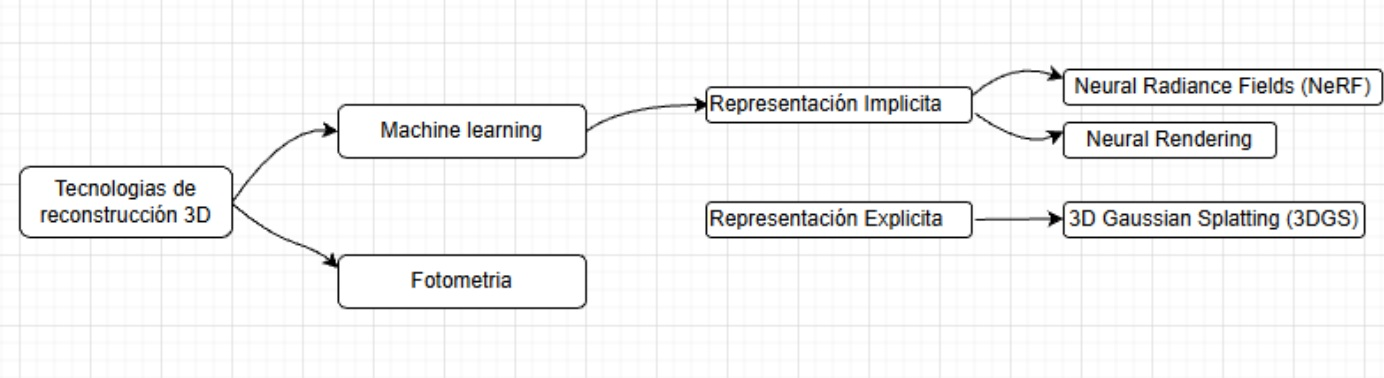
\includegraphics[width=0.9\textwidth]{figuras/figura2.1.jpg}
  \caption{Taxonomía.}
  \label{fig:taxonomia}
  \vspace{0.2cm}

  \small \textit{Fuente:} Elaboración propia.
\end{figure}

\section{Benchmarking}
En esta sección se tiene como punto el objetivo y la mejor metodología a seleccionar, y mediante el cual se definen los criterios de comparación basados en las ramas del árbol taxonómico (Autoconstrucción, Evaluación Estructural y Reconstrucción 3D).\par


\begin{table}[htbp]
  \centering
  \caption{Criterios de benchmarking para la selección metodológica}
  \label{tab:criterios-benchmarking}
  \small
  \setlength{\tabcolsep}{4pt}
  \renewcommand{\arraystretch}{1.2}
  \begin{tabular}{>{\raggedright\arraybackslash}p{0.26\textwidth} >{\raggedright\arraybackslash}p{0.26\textwidth} >{\raggedright\arraybackslash}p{0.38\textwidth}}
    \toprule
    \textbf{Eje de comparación} & \textbf{Criterio específico} & \textbf{Relevancia para la tesis} \\
    \midrule
    \textbf{I. Funcional (Autoconstrucción)} & Accesibilidad y usabilidad & ¿Es la herramienta utilizable por un no ingeniero, como un autoconstructor? \\
    & Enfoque en normativa local & ¿Aplica fórmulas simplificadas o normativas específicas para albañilería? \\
    & Integración de datos (input) & ¿Permite la entrada de datos mediante imágenes o requiere medidas manuales? \\
    \midrule
    \textbf{II. Tecnológico (Reconstrucción 3D)} & Tiempo de procesamiento & ¿Qué tiempo requieren la reconstrucción y el análisis en el equipo de procesamiento documentado? \\
    & Calidad y localización & ¿Con qué calidad se representan los elementos y con qué exactitud se localizan los hallazgos frente a las referencias? \\
    & Requerimientos de hardware & ¿Qué recursos de CPU, GPU y memoria requiere el procesamiento, separado de la captura con dron e iPhone? \\
    \bottomrule
  \end{tabular}
\end{table}

\subsection{Benchmarking funcional}

Esta sección compara las soluciones existentes que buscan dimensionar elementos estructurales, identificando la brecha de mercado en la Autoconstrucción.\par

\begin{table}[htbp]
  \centering
  \caption{Benchmarking funcional de herramientas para evaluación y predimensionamiento estructural}
  \label{tab:benchmarking-funcional}
  \scriptsize
  \setlength{\tabcolsep}{3pt}
  \renewcommand{\arraystretch}{1.15}
  \begin{tabular}{>{\raggedright\arraybackslash}p{0.16\textwidth} >{\raggedright\arraybackslash}p{0.16\textwidth} >{\raggedright\arraybackslash}p{0.15\textwidth} >{\raggedright\arraybackslash}p{0.25\textwidth} >{\raggedright\arraybackslash}p{0.20\textwidth}}
    \toprule
    \textbf{Herramienta/\newline Plataforma} & \textbf{Tipo de solución} & \textbf{Público objetivo} & \textbf{Metodología} & \textbf{Brecha identificada} \\
    \midrule
    ETABS, SAP2000 & Software de ingeniería (FEM) & Ingenieros estructurales & Análisis sísmico y de cargas detallado mediante cálculo avanzado. & No es accesible para el autoconstructor. Requiere meses de entrenamiento y licencias costosas. \\
    MathCAD / Excel & Hojas de cálculo / macros & Estudiantes y profesionales & Uso de fórmulas de predimensionamiento basadas en normas, como la RNE E.030, y áreas tributarias. & No es intuitivo; requiere la introducción manual de todos los datos, como áreas, luces y cargas, sin verificación visual. \\
    Apps genéricas de construcción, como calculadoras de hormigón & Aplicación móvil simple & Obreros y constructores & Calcula volúmenes de materiales o costos unitarios. & No aborda el predimensionamiento estructural, solo el metrado o el presupuesto. Carece de análisis de riesgo. \\
    \bottomrule
  \end{tabular}
\end{table}

\subsection{Benchmarking Tecnologico}

Esta es la sección se realizo la comparativa mediante el cua se justifica la elección de 3D Gaussian Splatting (3DGS) sobre su principal alternativa, Neural Radiance Fields (NeRF), y la fotogrametría tradicional.\par

\begin{table}[htbp]
  \centering
  \caption{Benchmarking tecnológico entre fotogrametría, NeRF y 3D Gaussian Splatting}
  \label{tab:benchmarking-tecnologico}
  \scriptsize
  \setlength{\tabcolsep}{3pt}
  \renewcommand{\arraystretch}{1.15}
  \begin{tabular}{>{\raggedright\arraybackslash}p{0.16\textwidth} >{\raggedright\arraybackslash}p{0.25\textwidth} >{\raggedright\arraybackslash}p{0.25\textwidth} >{\raggedright\arraybackslash}p{0.25\textwidth}}
    \toprule
    \textbf{Criterio} & \textbf{Fotogrametría (SfM/MVS)} & \textbf{Neural Radiance Fields (NeRF)} & \textbf{3D Gaussian Splatting (3DGS)} \\
    \midrule
    Representación & Malla (\textit{mesh}) o nube de puntos & Implícita (volumétrica/vóxeles) & Explícita (basada en puntos gaussianos 3D) \\
    Velocidad de entrenamiento & Media/alta (depende del tamaño) & Lenta y costosa (requiere optimización de red neuronal). & Muy rápida (más rápido que NeRF). \\
    Velocidad de \textit{rendering} & Rápida (basada en GPU) & Lenta (requiere consultar la red para cada rayo). & Tiempo real / interactivo (ideal para aplicaciones móviles y VR/AR). \\
    Requerimientos de cómputo & Dependen de las imágenes, la resolución y el método de reconstrucción. & Dependen del modelo, el entrenamiento y la resolución de consulta. & Se evaluarán para la optimización de la escena y el renderizado por separado; no se presupone ejecución en el dispositivo de captura. \\
    Precisión de profundidad & Alta (escalable, puede medir volúmenes). & Baja (a menudo genera profundidades imprecisas). & Media a alta (mejor que NeRF, pero la escalabilidad requiere pasos adicionales en la implementación). \\
    Calidad visual & Muy alta (texturas fotorrealistas). & Alta (excelente manejo de reflejos y luces). & Alta / superior (generalmente más nítido y con menos artefactos que NeRF). \\
    \bottomrule
  \end{tabular}
\end{table}

\section{Autoconstrucción de viviendas}

\subsection{Concepto y características principales}
Define la autoconstrucción de viviendas y sus principales características en el contexto urbano y periurbano.

\subsection{Autoconstrucción en contextos urbanos periurbanos}
Describe las particularidades de la autoconstrucción en zonas de expansión urbana, periferias y asentamientos con crecimiento progresivo.

\subsection{Riesgos estructurales asociados}
Explica los riesgos derivados de la informalidad constructiva, la falta de supervisión técnica, el uso inadecuado de materiales o el incumplimiento de normas.

\section{Evaluación estructural y métodos de inspección}

La autoconstrucción no constituye un fenómeno homogéneo; por el contrario, puede adoptar diversas formas dependiendo de factores socioeconómicos, culturales, territoriales y normativos. Estas variaciones determinan el grado de formalidad, el nivel técnico involucrado, la participación comunitaria y la calidad estructural de las edificaciones resultantes. El análisis de estas tipologías permite comprender los diferentes escenarios en los que se desarrolla la autoconstrucción y, por ende, identificar los puntos críticos que requieren herramientas de diagnóstico y asistencia técnica.\par

\subsection{Inspección estructural tradicional}
La modalidad más extendida en América Latina y el Perú es la autoconstrucción informal, donde las viviendas se levantan sin supervisión profesional, sin licencias municipales y sin aplicación rigurosa de normas técnicas. Sus características incluyen:\par

\begin{itemize}
  \item Ausencia de planos arquitectónicos, estructurales o sanitarios.
  \item Materiales adquiridos por disponibilidad, muchas veces de baja calidad o sin control de procedencia.
  \item Construcción por etapas en función del ahorro progresivo.
  \item Participación de maestros de obra empíricos o mano de obra no especializada.
  \item Intervenciones improvisadas, como ampliaciones o reforzamientos no calculados.
\end{itemize}

Esta modalidad incrementa la vulnerabilidad estructural, especialmente en zonas sísmicas, y constituye el núcleo del problema que aborda la presente investigación.\par

\subsection{Métodos de ensayos no destructivos (NDT)}
La autoconstrucción asistida surge como una alternativa intermedia entre la construcción informal y la vivienda formal. En ella, los usuarios participan activamente en el proceso constructivo, pero reciben acompañamiento técnico parcial proporcionado por arquitectos, ingenieros o entidades públicas/privadas. Este tipo de autoconstrucción puede incluir:\par

\begin{itemize}
  \item Revisión de planos básicos.
  \item Supervisión parcial en etapas críticas (cimientos, estructura, instalaciones).
  \item Orientación en compra de materiales.
  \item Programas municipales o estatales de asistencia (como ATHIS en Brasil o PCA en Perú).
\end{itemize}

Sin embargo, la cobertura de estos servicios sigue siendo limitada y no responde a la escala del déficit habitacional.\par

\subsection{Necesidad de métodos digitales automatizados}
Es aquella que se desarrolla por fases, según la disponibilidad de recursos económicos y mano de obra. Se caracteriza por:\par

\begin{itemize}
  \item Construcción inicial de núcleos básicos (primer piso, un ambiente, servicios mínimos).
  \item Ampliaciones verticales o horizontales con el tiempo.
  \item Cambios de uso o redistribuciones sucesivas.
\end{itemize}

Debido a su naturaleza incremental, estas viviendas suelen presentar irregularidades geométricas y ausencia de continuidad estructural, lo que aumenta la dificultad para realizar inspecciones manuales.\par

\subsection{Autoconstrucción planificada}
A diferencia de la informal, esta modalidad incluye planificación previa y uso de manuales, guías o modelos estandarizados, aunque todavía conserva participación directa del usuario. Es común en países del Norte Global, donde existen sistemas de self-build housing regulados. Sus características incluyen:\par

\begin{itemize}
  \item Asesoría técnica obligatoria.
  \item Acceso a prototipos estructurales validados.
  \item Normativas que permiten construir con acompañamiento supervisado.
  \item Cooperativas o asociaciones comunitarias de autoconstructores.
\end{itemize}

Aunque más segura, esta modalidad es poco común en el contexto peruano.\par

\subsection{Participación comunitaria y autoayuda mutua}
En muchas zonas rurales y periurbanas, la autoconstrucción se basa en redes de cooperación donde vecinos y familiares aportan mano de obra de manera recíproca. Este sistema, conocido como minga, faena o mano vuelta, tiene características distintivas:\par

\begin{itemize}
  \item Trabajo colectivo organizado.
  \item Uso de saberes tradicionales.
  \item Optimización de tiempos y reducción de costos.
  \item Mayor cohesión social, aunque sin garantía técnica.
\end{itemize}

Si bien fortalece la construcción comunitaria, no garantiza seguridad estructural.\par

\chapter{Análisis del problema}

\section{Antecedentes relativos al contexto peruano}
La autoconstrucción representa el mecanismo predominante de acceso a la vivienda en el Perú, configurando el panorama urbano nacional. Investigaciones recientes demuestran que aproximadamente el 71\% de las viviendas en zonas urbanas se han edificado mediante este sistema, concentrándose principalmente en las periferias limeñas y ciudades emergentes donde la oferta formal resulta insuficiente.\par

Los índices de informalidad revelan cifras alarmantes: apenas el 16\% cuenta con licencia municipal y solo el 14\% recibe asesoría técnica calificada. Esta realidad se traduce en condiciones estructurales precarias: 47\% de techos vulnerables, 30\% de muros deficientes y 12\% de pisos inadecuados según estándares técnicos.\par

La ubicación sísmica del país agrava esta situación. Estadísticas oficiales indican que más del 60\% de estas construcciones nunca ha sido evaluado técnicamente, generando un riesgo latente ante desastres naturales.\par

Ante esta problemática, emergen propuestas de asistencia técnica como el Programa de Construcción Asistida en Carabayllo y experiencias similares en Tacna de parte de su Municipalidad provincial, aunque su alcance sigue siendo limitado.\par

\begin{figure}[htbp]
  \centering
  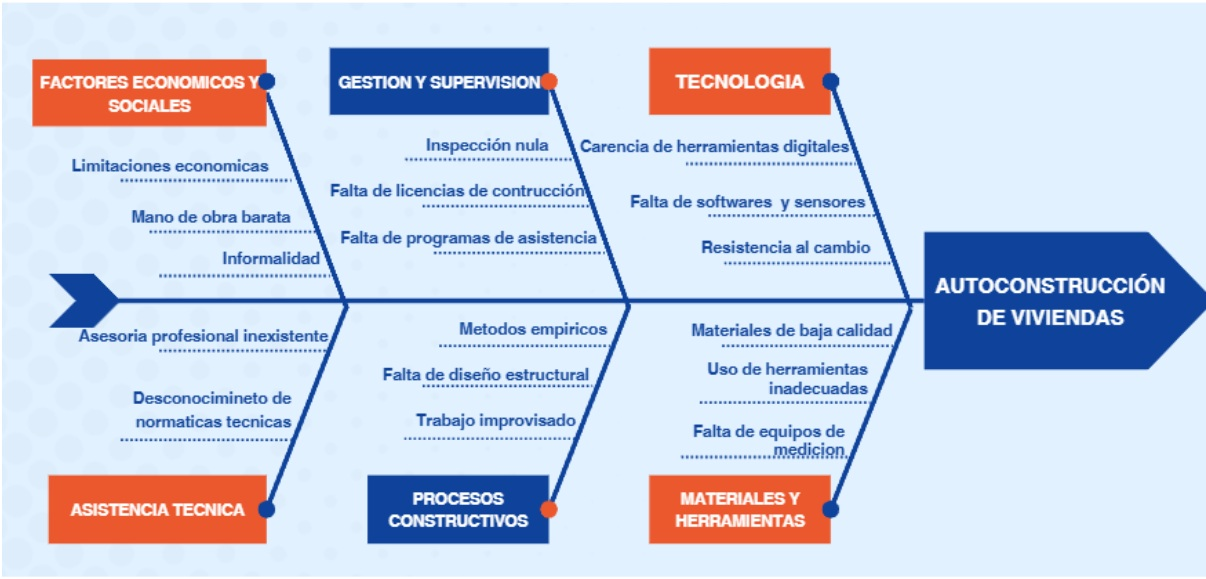
\includegraphics[width=0.9\textwidth]{figuras/figura4.1.jpg}
  \caption{Diagrama de Ishikawa.}
  \label{fig:diagrama-ishikawa}
  \vspace{0.2cm}

  \small \textit{Fuente:} Elaboración propia.
\end{figure}

\section{Actores que intervienen en la problemática}
El proceso de evaluación estructural de viviendas autoconstruidas involucra distintos actores técnicos, institucionales y sociales, cuyas decisiones y capacidades influyen directamente en la seguridad estructural del parque habitacional.\par

\begin{figure}[htbp]
  \centering
  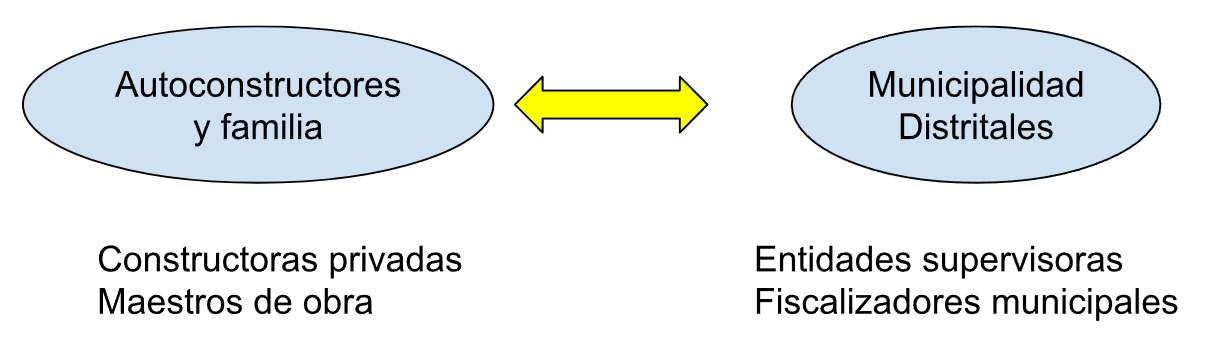
\includegraphics[width=0.9\textwidth]{figuras/figura4.2.jpg}
  \caption{Diagrama de Ishikawa.}
  \label{fig:diagrama-ishikawa-actores}
  \vspace{0.2cm}

  \small \textit{Fuente:} Elaboración propia.
\end{figure}



\subsection{Familias peruanas (Autoconstrucción)}
Las familias peruanas que optan por la autoconstrucción representan el núcleo del problema, actuando como gestores y ejecutores de sus propias viviendas, generalmente sin acceso a asesoría técnica formal.\par

Motivadas por la necesidad habitacional urgente y limitaciones económicas, recurren a conocimientos empíricos, mano de obra familiar o de maestros de obra no especializados.\par

Además de materiales de calidad variable, lo que genera diseños estructurales inadecuados, falta de refuerzos esenciales y ausencia de cumplimiento normativo, incrementando significativamente la vulnerabilidad sísmica de sus viviendas y exponiéndose a riesgos de colapso ante desastres naturales.\par

\subsection{Autoridades municipalidades}

Las municipalidades distritales, como entidades responsables de supervisar y fiscalizar las construcciones en su jurisdicción, enfrentan serias limitaciones operativas que impiden un control efectivo de la autoconstrucción.\par

Ellos hacen uso de equipos técnicos reducidos, insuficiente especialización en ingeniería estructural y recursos tecnológicos escasos, su capacidad de inspección se restringe a revisiones visuales superficiales, dejando sin detectar la mayoría de las deficiencias estructurales críticas en viviendas autoconstruidas, lo que perpetúa la informalidad y el riesgo en el parque habitacional.\par


\chapter{Diseño y desarrollo de la solución}

\section{Alcance funcional del MVP}

El alcance funcional del prototipo SE-PEAV se organiza según los componentes necesarios para cumplir los cinco objetivos específicos. La clasificación siguiente establece compromisos de desarrollo y evaluación; no representa una declaración de que los componentes ya se encuentren implementados o validados. Cada componente deberá acompañarse de evidencias de ejecución y resultados verificables.\par

\begin{table}[htbp]
  \centering
  \caption{Componentes y alcance de evaluación del prototipo}
  \label{tab:clasificacion-mvp}
  \small
  \setlength{\tabcolsep}{4pt}
  \renewcommand{\arraystretch}{1.2}
  \begin{tabular}{>{\raggedright\arraybackslash}p{0.22\textwidth} >{\raggedright\arraybackslash}p{0.68\textwidth}}
    \toprule
    \textbf{Clasificación} & \textbf{Componentes considerados} \\
    \midrule
    Datos de campo & Captura exterior con dron e interior con iPhone; fotografías y videos RGB; selección y preprocesamiento; metadatos; anotaciones revisadas y particiones por vivienda. \\
    Núcleo tecnológico & Reconstrucción mediante 3D Gaussian Splatting; identificación de deficiencias mediante inteligencia artificial y asociación de detecciones con la representación tridimensional. \\
    Servicios de soporte & API para proyectos e inspecciones; persistencia y almacenamiento de evidencias; visor web y generación de reportes con hallazgos trazables. \\
    Evaluación & Datos de referencia; pruebas de integración; métricas de reconstrucción, detección, localización y tiempo de procesamiento; configuración y procedimiento reproducibles. \\
    Fuera del alcance & Captura LiDAR, aplicación móvil completa y despliegue en producción. \\
    \bottomrule
  \end{tabular}
\end{table}

\section{Herramientas y entorno de desarrollo}

En esta sección se describen las tecnologías y herramientas del prototipo SE-PEAV. Los dispositivos de adquisición se distinguen del entorno de cómputo: el dron y el iPhone capturarán los registros visuales, mientras que la reconstrucción y la inferencia se ejecutarán en el equipo de procesamiento o servidor documentado para los experimentos. No se establece como requisito ejecutar estos procesos en el teléfono o en el dron.

\subsection{Desarrollo del backend}
El backend del sistema se implementó utilizando el lenguaje de programación \textbf{Python 3.12}, seleccionado por su madurez y amplio ecosistema para el desarrollo de inteligencia artificial y procesamiento tridimensional. Las principales herramientas y bibliotecas utilizadas son:
\begin{itemize}
    \item \textbf{FastAPI (v0.109.0):} Framework web asíncrono de alto rendimiento para la creación de la API REST que gestiona las peticiones de los clientes (móvil y web).
    \item \textbf{SQLAlchemy y Alembic:} Para el mapeo objeto-relacional (ORM) y el control de migraciones de la base de datos relacional PostgreSQL.
    \item \textbf{Celery (v5.3.6):} Gestor de colas de tareas asíncronas para el procesamiento diferido y pesado de la reconstrucción tridimensional y el análisis mediante IA.
    \item \textbf{OpenCV, Open3D y Trimesh:} Bibliotecas clave para el procesamiento de imágenes, manipulación de nubes de puntos densas e interpolación de mallas estructurales tridimensionales.
\end{itemize}

\subsection{Infraestructura de almacenamiento y contenedores}
Para garantizar la portabilidad y escalabilidad de la solución en entornos locales y en la nube (como Google Cloud Platform), el sistema utiliza las siguientes herramientas de infraestructura:
\begin{itemize}
    \item \textbf{Docker y Docker Compose:} Herramientas de contenedorización que encapsulan los servicios de la aplicación (API Backend, Celery Workers, base de datos PostgreSQL, Redis y MinIO) asegurando consistencia entre desarrollo y producción.
    \item \textbf{Redis (v5.0.1):} Utilizado como intermediario de mensajería (broker) de alto rendimiento para la orquestación de tareas en Celery.
    \item \textbf{MinIO / Amazon S3:} Servidor de almacenamiento de objetos local compatible con la API de AWS S3, utilizado para resguardar los videos capturados, frames extraídos, nubes de puntos PLY y reportes técnicos en formato PDF.
\end{itemize}

\subsection{Dispositivos de captura y presentación visual}
El flujo previsto comprende dos fuentes de adquisición y un entorno de consulta:
\begin{itemize}
    \item \textbf{Captura exterior con dron:} Registro de las fachadas y demás superficies exteriores visibles incluidas en el recorrido de adquisición. Se documentarán el equipo, la cámara, los parámetros de captura y las zonas cubiertas o no observadas.
    \item \textbf{Captura interior con iPhone:} Registro de los ambientes y elementos interiores seleccionados mediante fotografías y videos RGB. Se documentarán el modelo del teléfono, la lente y la aplicación utilizada. El procedimiento no requiere desarrollar una aplicación móvil propia ni presupone disponer de profundidad o telemetría.
    \item \textbf{Visor web:} Presentación de las representaciones tridimensionales y los hallazgos asociados, con acceso a la imagen de origen y a su identificación como captura exterior o interior. Se verificará la compatibilidad del visor basado en Three.js con el formato de representación utilizado; la visualización de una nube de puntos no se considerará por sí sola equivalente al renderizado de gaussianas.
\end{itemize}

\section{Arquitectura de la solución}

La arquitectura del sistema SE-PEAV se basa en un diseño modular por capas que separa las responsabilidades de captura de datos, ingestión, procesamiento por lotes en segundo plano, análisis inferencial e interfaces de presentación.

\subsection{Transferencia, organización e ingesta de datos}
El flujo de carga se define independientemente del dispositivo utilizado para capturar las imágenes. Los archivos podrán transferirse previamente a una computadora o cargarse desde un cliente compatible. La conexión directa del dron o del iPhone con la API no se considera un requisito. La ruta de transferencia efectivamente utilizada se documentará en cada sesión:
\begin{enumerate}
    \item Identificar la vivienda y las sesiones exterior e interior; organizar los archivos originales y conservar sus metadatos disponibles.
    \item Registrar la inspección y solicitar desde el cliente de carga un destino de almacenamiento autorizado por la API.
    \item Transferir las fotografías o videos al almacenamiento de objetos, verificar su integridad y registrar el dispositivo, la sesión, la zona y los parámetros de adquisición disponibles.
    \item Extraer fotogramas cuando corresponda y aplicar la selección y el preprocesamiento documentados, manteniendo la relación entre cada imagen derivada y su archivo original.
    \item Registrar los datos preparados y programar las tareas de reconstrucción e inferencia en el entorno de procesamiento.
\end{enumerate}

\subsection{Diagrama de componentes e interacción}
El pipeline de procesamiento se divide en cuatro capas operativas esenciales:
\begin{itemize}
    \item \textbf{Capa de ingesta:} Recibirá fotografías y videos de las sesiones exteriores e interiores. Aplicará extracción de fotogramas, selección y control de calidad con parámetros documentados, conservando los originales y la trazabilidad de cada transformación.
    \item \textbf{Motor de reconstrucción:} Empleará Structure from Motion (SfM) con COLMAP para estimar parámetros y poses de cámara y obtener una representación inicial, seguida de la optimización de la escena mediante 3D Gaussian Splatting. Las imágenes del dron y del iPhone se identificarán por cámara y configuración. Las reconstrucciones conservarán su sistema de coordenadas; su eventual unificación requerirá un procedimiento de alineación evaluado.
    \item \textbf{Capa de análisis y localización:} Aplicará el modelo de detección o segmentación seleccionado, considerando YOLOv8 como candidato, a fotografías y fotogramas. La versión, las categorías, los pesos y el eventual ajuste se documentarán. Un módulo de correspondencia utilizará las poses de cámara y la geometría disponible para asociar detecciones con la representación 3D; registrará las asociaciones verificables y los casos no localizables. Los criterios técnicos distinguirán la norma E.060, Concreto Armado, de la E.070, Albañilería, según el elemento analizado \citep{rneportal}. No se declarará la verificación de espesores, distancias o cumplimiento normativo sin las medidas de referencia y el procedimiento correspondiente.
    \item \textbf{Capa de reportes:} Reunirá los hallazgos, las imágenes de origen, la localización disponible y las limitaciones observadas en un reporte enlazado con el visor. Cualquier clasificación preliminar de vulnerabilidad requerirá criterios y validación documentados; no se asumirá que una detección visual equivale a un diagnóstico de riesgo estructural.
\end{itemize}

\subsection{Correspondencia entre exterior e interior}
El identificador de vivienda relacionará ambas capturas desde la adquisición hasta el reporte. Antes de elegir una reconstrucción conjunta o modelos separados se evaluará la disponibilidad de correspondencias y referencias comunes. El procedimiento elegido deberá documentar cómo se relacionan las coordenadas, cómo se establece la escala cuando se realicen mediciones y con qué error se alinean los modelos. Si no se demuestra una alineación suficiente, el visor presentará las reconstrucciones identificadas por zona, sin sugerir continuidad geométrica verificada.

\subsection{Evaluación diferenciada del flujo}
El protocolo distinguirá la calidad de reconstrucción exterior e interior, el desempeño del detector en imágenes y la exactitud de la localización tridimensional. Los tiempos de transferencia, preparación, reconstrucción, inferencia y generación de reportes se registrarán por separado. Las anotaciones de referencia y las comprobaciones de localización permitirán evaluar cada etapa sin atribuir al detector errores que provengan de la reconstrucción o de la asociación espacial.

\section{Implementación de servicios backend}

La capa de servicios backend de la API REST fue estructurada bajo una arquitectura limpia en FastAPI. Los principales endpoints e implementaciones lógicas desarrolladas son:
\begin{itemize}
    \item \textbf{Servicio de Autenticación (\texttt{/auth}):} Implementa registro de usuarios, login con hashing de contraseñas mediante \texttt{bcrypt} y generación de tokens de seguridad JWT persistentes.
    \item \textbf{Servicio de Proyectos (\texttt{/projects}):} Permite la creación, lectura y listado georreferenciado de los proyectos de inspección asignados a cada ingeniero.
    \item \textbf{Servicio de Inspecciones (\texttt{/inspections}):} Gestiona el ciclo de vida de una inspección, controlando los estados de procesamiento (\texttt{PENDING}, \texttt{PROCESSING}, \texttt{COMPLETED}, \texttt{FAILED}) y exponiendo endpoints de consulta para las detecciones de fallas y métricas estructurales calculadas.
    \item \textbf{Servicio de Reportes (\texttt{/reports}):} Genera y sirve el archivo de reporte final en formato PDF, además de enlazar dinámicamente con el visor tridimensional interactivo mediante la ruta \texttt{/viewer/\{inspection\_id\}}.
\end{itemize}

\chapter{Discusión, conclusiones y recomendaciones}

\section{Discusión}
Interpreta los resultados de la solución propuesta, sus alcances, limitaciones y relación con los trabajos revisados en el estado del arte.

\section{Conclusiones}

\subsection{Conclusión general}
Redacta una conclusión global directamente vinculada con el objetivo general de la tesis.

\subsection{Conclusiones específicas}

\subsubsection{Objetivo específico 1}
Redactar la conclusión sobre las deficiencias seleccionadas, los requisitos de información y los criterios de evaluación definidos, sustentándola en los resultados del primer objetivo.

\subsubsection{Objetivo específico 2}
Redactar la conclusión sobre la construcción y calidad del conjunto de datos exterior capturado con dron e interior capturado con iPhone, indicando su composición, preparación, anotación y limitaciones.

\subsubsection{Objetivo específico 3}
Redactar la conclusión sobre el procedimiento de reconstrucción tridimensional implementado y su capacidad para representar y localizar los elementos de interés.

\subsubsection{Objetivo específico 4}
Redactar la conclusión sobre la integración del modelo de inteligencia artificial y la asociación de las detecciones con la representación tridimensional, a partir de evidencias verificables.

\subsubsection{Objetivo específico 5}
Redactar la conclusión sobre el desempeño medido del prototipo, relacionando las métricas obtenidas con los datos de referencia, los criterios de evaluación y las condiciones de las pruebas.

\subsection{Limitaciones}
La discusión de las limitaciones deberá sustentarse en la captura y la evaluación efectivamente realizadas. Se documentarán el número y la diversidad de viviendas, la distribución de las categorías de deficiencias, la calidad de las anotaciones, las condiciones de captura y los recursos computacionales utilizados. También se identificarán los casos en que la reconstrucción, la detección o la asociación espacial de hallazgos no satisfagan los criterios establecidos.\par

Las conclusiones se limitarán a las categorías, viviendas y condiciones evaluadas. La verificación de los servicios de software y la ejecución de un caso de integración no sustituirán la evaluación del desempeño de la reconstrucción tridimensional y la inteligencia artificial. Los hallazgos del prototipo se interpretarán como apoyo a una evaluación preliminar y no como un dictamen estructural definitivo.\par

\subsection{Recomendaciones y trabajos futuros}
Las recomendaciones finales se formularán a partir de los resultados y las limitaciones observadas. Como posibles ampliaciones fuera del alcance actual se consideran una aplicación móvil completa para captura guiada, la incorporación de sensores LiDAR, la evaluación en nuevas localidades y categorías de deficiencias, los estudios de usabilidad con usuarios finales y el despliegue en producción. Su pertinencia y prioridad deberán justificarse con la evidencia obtenida.\par

La captura de datos reales, la reconstrucción mediante 3D Gaussian Splatting, la integración de inteligencia artificial y la evaluación de su desempeño forman parte de los objetivos de esta investigación y no se trasladan a trabajos futuros.\par

% Se conservan las dos referencias existentes durante la migración a BibTeX.
% Las demás citas manuales requieren verificar e incorporar su fuente completa.
\nocite{kerbl2023,mildenhall2020}
\bibliographystyle{apalike}
\begingroup
\raggedright
\bibliography{referencias}
\endgroup

\appendix

\chapter{Matriz de consistencia}
Incluye aquí la matriz de consistencia de la investigación.

\chapter{Instrumentos de recolección de datos}
Los instrumentos siguientes constituyen la estructura prevista para documentar la adquisición y preparación de los datos. Se completarán durante las sesiones de captura y el procesamiento; no representan registros de campo ya obtenidos.

\section{Ficha de identificación de vivienda y sesiones}
La ficha registrará el identificador de vivienda, la fecha, el responsable, los ambientes o superficies seleccionados y las condiciones de acceso. Cada sesión tendrá un código asociado a la vivienda y se clasificará como exterior con dron o interior con iPhone. Se identificarán las zonas cubiertas, las zonas no observadas y las incidencias que limiten la interpretación de las imágenes.

\section{Protocolo de captura exterior con dron}
Antes de la sesión se definirán las superficies de interés y el recorrido previsto. La ficha de captura registrará el modelo del dron y de su cámara, la modalidad de adquisición, la resolución, la lente, los parámetros disponibles y la relación entre archivos y zonas observadas. Se comprobarán cobertura, nitidez, iluminación y continuidad visual entre tomas. Las distancias, alturas y demás parámetros efectivamente utilizados se consignarán en el registro de campo, sin asumir valores no medidos.

\section{Protocolo de captura interior con iPhone}
La sesión se organizará por ambientes y elementos de interés. Se registrarán modelo del iPhone, aplicación, lente, resolución, modalidad de captura y condiciones de iluminación. El recorrido buscará conservar cobertura y continuidad visual, identificando cambios de cámara o configuración. Los registros corresponden a fotografías y videos RGB; no se considerarán datos de profundidad o LiDAR como entrada del procedimiento previsto.

\section{Registro de preparación y control de calidad}
El registro vinculará cada fotografía o fotograma con su archivo original, sesión, vivienda y zona. Para videos se documentarán el criterio de extracción y la marca temporal de los fotogramas. Se consignarán selección o descarte y su motivo, transformaciones aplicadas y versión del conjunto. Se revisarán imágenes borrosas, exposición inadecuada, oclusiones y cobertura insuficiente. La selección procurará conservar vistas útiles para la reconstrucción y evidencia suficiente para la anotación.

\section{Ficha de anotación y referencia}
Cada anotación registrará imagen de origen, categoría de deficiencia, ubicación en la imagen, autor, revisión técnica e incertidumbre. Las reglas de anotación y el tratamiento de casos ambiguos se documentarán antes de evaluar el detector. Las medidas o puntos de referencia utilizados para comprobar geometría y localización tendrán un registro del método y de las condiciones de obtención. Los hallazgos sin correspondencia 3D verificable conservarán su evidencia 2D y se identificarán como no localizados.

\section{Organización y particiones de datos}
Se elaborará un inventario por vivienda, sesión, zona, dispositivo y categoría anotada. Los registros interiores y exteriores de una misma vivienda permanecerán en una única partición para la evaluación del detector. Se documentarán por separado las imágenes de cada escena destinadas a optimizar la reconstrucción y las reservadas para evaluar nuevas vistas. Los equipos, parámetros de captura, cantidad de viviendas, distribución de categorías y criterios de aceptación se precisarán en el protocolo previo a la evaluación.

\chapter{Caso de prueba mínimo reproducible}

Este caso de prueba mínimo reproducible constituye una prueba auxiliar de integración de los servicios de software. Utiliza datos preparados y hallazgos controlados para verificar el registro, la persistencia, el almacenamiento, la visualización y la generación de reportes. Su ejecución no sustituye la captura de datos reales ni acredita el cumplimiento de los objetivos de reconstrucción tridimensional, identificación mediante inteligencia artificial y evaluación del desempeño. Estos objetivos requieren pruebas adicionales con datos de campo, referencias documentadas y métricas definidas previamente.\par

La entrada del caso estará compuesta por un proyecto de prueba, una inspección asociada, evidencias visuales controladas y un conjunto de hallazgos definidos en formato estructurado. El flujo esperado comprende la creación del proyecto, el registro de la inspección, la asociación de evidencias, la ejecución del análisis simplificado, la consulta de resultados, la apertura del visor y la generación del reporte técnico. El caso se considerará aceptado cuando el sistema produzca salidas consistentes y reproducibles: registros persistidos, evidencias asociadas, resultado preliminar trazable, visor con datos del caso y reporte generado desde la información de la inspección.\par

\begin{longtable}{>{\raggedright\arraybackslash}p{0.28\textwidth} >{\raggedright\arraybackslash}p{0.62\textwidth}}
  \caption{Ficha del caso de prueba mínimo reproducible}
  \label{tab:caso-prueba-minimo}\\
  \toprule
  \textbf{Campo} & \textbf{Descripción} \\
  \midrule
  \endfirsthead
  \toprule
  \textbf{Campo} & \textbf{Descripción} \\
  \midrule
  \endhead
  Nombre del caso & Inspección controlada de vivienda autoconstruida con evidencias simuladas y análisis simplificado. \\
  Objetivo & Verificar que el MVP permite registrar una inspección, persistir datos, asociar evidencias, visualizar hallazgos, calcular un resultado preliminar trazable y generar un reporte técnico reproducible. \\
  Entrada & Proyecto de vivienda controlada, inspección asociada, conjunto de imágenes o evidencias de prueba, archivo JSON con hallazgos simulados o controlados, parámetros básicos del análisis y metadatos del inmueble. \\
  Datos y evidencias necesarias & JSON de proyecto, JSON de inspección, imágenes controladas o referencias documentadas, registros en PostgreSQL, objeto o ruta de storage, respuesta de API, captura del visor, tabla de score y reporte HTML/PDF generado. \\
  Flujo esperado & Crear proyecto; crear inspección; cargar o registrar evidencias; guardar metadatos; ejecutar análisis simplificado; consultar resultados; abrir visor conectado a la inspección; generar reporte; conservar capturas y archivos de salida. \\
  Salidas esperadas & Registro persistido de proyecto e inspección, evidencias asociadas, resultado de vulnerabilidad preliminar, visor con datos del caso, reporte técnico generado y conjunto de capturas para anexos. \\
  Criterios de aceptación & La API responde correctamente; la inspección queda persistida; las evidencias quedan registradas o documentadas; el análisis produce un score trazable; el visor muestra datos del caso; el reporte se genera desde los datos de la inspección; el flujo puede repetirse con los mismos datos controlados. \\
  Evidencia a capturar & Captura Swagger/Postman, consulta de base de datos, captura o ruta de storage, JSON de entrada, JSON de salida, captura del visor, tabla de criterios de análisis, reporte generado y breve guion de reproducción. \\
  \bottomrule
\end{longtable}

\chapter{Material complementario}
Incluye capturas, diagramas, configuraciones, tablas adicionales o evidencias del desarrollo de la solución.

\end{document}
